% interacttfosample.tex
% v1.01 - May 2016

\documentclass[]{interact}

\usepackage[utf8]{inputenc}% TODO: возможно, убрать. Когда русского текста не останется
%\usepackage{supertabular}% TODO: избавиться
\usepackage{hhline}% TODO: избавиться, переписав таблицы
\usepackage{array}% TODO: избавиться
\usepackage{color}% TODO: избавиться
\makeatletter
\newcommand\arraybslash{\let\\\@arraycr}
\makeatother


\usepackage{epstopdf}% To incorporate .eps illustrations using PDFLaTeX, etc.
\usepackage{subfigure}% Support for small, `sub' figures and tables
\usepackage[english,russian]{babel}
\usepackage[numbers,sort&compress,merge]{natbib}% Citation support using natbib.sty
\bibpunct[, ]{[}{]}{,}{n}{,}{,}% Citation support using natbib.sty
\renewcommand\bibfont{\fontsize{10}{12}\selectfont}% Bibliography support using natbib.sty

\theoremstyle{plain}% Theorem-like structures
\newtheorem{theorem}{Theorem}[section]
\newtheorem{lemma}[theorem]{Lemma}
\newtheorem{corollary}[theorem]{Corollary}
\newtheorem{proposition}[theorem]{Proposition}

\theoremstyle{definition}
\newtheorem{definition}[theorem]{Definition}
\newtheorem{example}[theorem]{Example}

\theoremstyle{remark}
\newtheorem{remark}{Remark}
\newtheorem{notation}{Notation}

\begin{document}

\articletype{REGULAR ARTICLE}

\title{Oscillator strengths for Rydberg states in NaHe}

\author{
\name{Anastasia S. Chervinskaya, Sergei V. Elfimov, Dmitrii L. Dorofeev, Boris A. Zon}
\affil{Voronezh State University, 394006 Voronezh, Russia
}
}

\maketitle

\begin{abstract}
With the help of a semi-analytical procedure the oscillator strengths for Rydberg electronic transitions in NaHe molecule are calculated which account for the effects of l-coupling (due to dipole potential of the core). Such effects result in non-zero oscillator strength values for some transitions which are forbidden in the widely used atom-like model of molecular Rydberg states. For the allowed transitions we also report the difference between the atom-like calculations and the calculations which take into account the dipole moment of the molecular core in the frame of one-channel theory.
\end{abstract}

\begin{keywords}
Rydberg states; Oscillator strengths; NaHe;
\end{keywords}


\section{Введение}
Спектроскопия высоковозбужденных состояний представляет собой важную область атомной и молекулярной спектроскопии. Высоковозбужденными считают состояния, энергии которых близки к энергиям ионизации системы.
Также такие состояния называют ридберговскими. Такие состояния допускают эффективное описание в одночастичном приближении, при котором один из электронов, так называемый ридберговский электрон, обладает большой энергией и движется в поле потенциала атомного или молекулярного остова. В поле остова доминирует монопольный кулоновский потенциал, тогда как вклад высших мультипольных компонент относительно невелик. По этой причине состояние ридберговского электрона близко к водородоподобному, отличие от которого характеризуется поправкой к главному квантовому числу ридберговского электрона, называемой квантовым дефектом. Таким образом, именно анализ квантовых дефектов ридберовских состояний позволяет получить информацию о свойствах остова системы[1].
Лазерная абляция в металлах недавно сделала возможным погружение атомов различных металлов и небольших кластеров таких атомов в гелиевые нанокапли. Их спектры определяются с использованием лазерно-индуцированной флюоресценции.
За прошедшие годы были получены и исследованы в инфракрасной и видимой области различные молекулы в гелиевых каплях, начиная с ионов металла до больших органических молекул, а также ряд Ван-дер-Вальсовых комплексов и даже большие кластеры металла. Комплексы MHe+ (M=Li, Na, K) представляют большой интерес. Их изучение важно для понимания процессов, происходящих в плазме, явления нуклеации, фазовых переходов и структур, образующихся в атмосфере[6].
Теоретическое описание атомных и молекулярных ридберговских состояний весьма важна для интерпретации спектров астрономических объектов[3], в особенности инфракрасной части спектра. В лабораторных условиях ридберговские состояния получают вплоть до значений главного квантового числа $n\approx300$[4]. Высокая чувствительность ридберговских состояний к внешним полям и их дальнодействующие взаимодействия являются очень привлекательными для технологических приложений, например, таких как квантовые вычисления[5].

Теория квантового дефекта (Quantum Defect Theory - QDT) является наиболее удобным методом исследования ридберговских состояний. QDT находит широкое применение в самых различных приложениях атомно- молекулярной спектроскопии, от идентификации спектроскопических данных и высокоточных методов расчетов потенциала ионизации, до описания автоионизации и рассеяния электронов на атомах и ионах. В формализме QDT считается, что ридберговский электрон большую часть времени проводит вдали от атомного или молекулярного остова на расстоянии $r$, значительно превышающем характерный радиус остова $r_c$. При этом взаимодействие электрона с остовом можно считать почти кулоновским; его отличие от кулоновского возникает лишь при $r<r_c$ и учитывается квантовым дефектом, входящим в формулу Ридберга для энергетических уровней:


\begin{equation}
E=-\frac{Z^2}{2\nu^2}=-\frac{Z^2}{2\left(n-\mu\right)^2}
\end{equation}

В работах Бейтса и Дамгаард был предложен метод расчета сил осцилляторов связанных состояний для простых атомных систем. Таким образом, метод QDT дает также возможность простого расчета сил осцилляторов для электронных переходов, что и было использовано в настоящей работе
Альтернативный QDT метод вычисления сил осцилляторов связан с использованием модельного потенциала, впервые предложенного в работах Simons (1971) и Martin (1975).
Ридберговский электрон с достаточно большим угловым моментом значительную часть времени проводит на далеком расстоянии от молекулярного остова. Поэтому на движение электрона оказывают влияние лишь дальнодействующие компоненты остовного потенциала. Эта концепция известна как модель дальнего взаимодействия (long-range interaction model). Кроме кулоновского поля молекулярного остова, роль такого дальнодействующего потенциала в полярных молекулах будет играть дипольный момент остова. Поэтому теория ридберговских состояний в полярных молекулах должна быть основана на корректном учете дипольного момента остова[2].
К сожалению, традиционные техники компьютерного расчета атомных систем (решения уравнений Хартри-Фокка и т.д.) являются неэффективными для расчета спектра и волновых функций высоковозбужденных состояний. Из-за этого необходимо пользоваться техникой, основанной на методе квантового дефекта[7].







\section{Прямое приближение Борна-Оппенгеймера}

Движение электрона в непроникающем ридберговском состоянии описывается его дальнодействующим взаимодействием с остовом, а именно, взаимодействием с кулоновским потенциалом, комбинированным с потенциалом свободно вращающегося диполя. Для анализа этого взаимодействия мы будем использовать приближение Борна-Оппенгеймера, применимое, когда диполь покоится или медленно движется по сравнению с движением электрона. Показано, что в данном приближении можно разделить радиальные и угловые переменные и в явном виде записать решение уравнения Шредингера для ридберговского электрона.
Сразу поговорим о границах применимости такого приближения. В прямом приближении Борна-Оппенгеймера момент импульса ридберговского электрона сильно связан с осью симметрии остова. Это имеет место, когда прецессия орбиты ридберговского электрона имеет более высокую частоту, чем вращение молекулы в целом.[8]
\begin{equation}
4BJ\ll|\Delta E_{qd}|=\frac{\mu}{\nu^3}
\end{equation}
С учетом дипольного взаимодействия мы можем записать гамильтониан ридберговской системы таким образом:
\begin{equation}
H=-\frac{\Delta}{2}-\frac{1}{r}+\frac{{\bf dr}}{r^3} 
\end{equation}


\section{Глава 1. Прямое
приближение
Борна-Оппенгеймера.}
\subsection{1.1
Приближение Борна-Оппенгеймера. Границы
применимости.}
Движение электрона в непроникающем ридберговском состоянии описывается его дальнодействующим взаимодействием с остовом, а именно, взаимодействием с кулоновским потенциалом, комбинированным с потенциалом свободно вращающегося диполя. Для анализа этого взаимодействия мы будем использовать приближение Борна-Оппенгеймера, применимое, когда диполь покоится или медленно движется по сравнению с движением электрона. Показано, что в данном приближении можно разделить радиальные и угловые переменные и в явном виде записать решение уравнения Шредингера для ридберговского электрона.

Сразу поговорим о границах применимости такого приближения. В прямом приближении Борна-Оппенгеймера момент импульса ридберговского электрона сильно связан с осью симметрии остова. Это имеет место, когда прецессия орбиты ридберговского электрона имеет более высокую частоту, чем вращение молекулы в целом.[8]

\begin{equation*}
4\mathit{BJ}{\ll}\left|{\Delta}E_{\mathit{qd}}\right|=\frac{\mu }{n^3}(1.1)
\end{equation*}
Здесь  $B$ -
вращательная константа в операторе центробежной энергии ядер

\begin{equation*}
	H^{+}=B\widehat  N^2(1.2)
\end{equation*}
$J$ -- полный момент молекулы (исключая спин ридберговского электрона),
$n$ -- главное квантовое число,
$\nu$ -- квантовый дефект.

\begin{equation*}
E_n=\frac{-1} 2\left(n-\mu \right)^{-2}(1.3)
\end{equation*}
\begin{equation*}
{\Delta}E_{\mathit{qd}}= \frac {|\mu|} {n^3}(1.4)
\end{equation*}
сдвиг энергии уровня.

\subsection{1.2 Задача о
ридберговском электроне в кулон-дипольном
потенциале.}
С учетом дипольного взаимодействия мы можем записать гамильтониан ридберговской системы таким образом:

\begin{equation*}
\widehat  H=\frac{-{\Delta}} 2-\frac 1 r+\frac{\mathit{dr}}{r^3}(2.1)
\end{equation*}
При выборе сферической системы координат,
в которой ось \foreignlanguage{english}{z}
сонаправлена с направлением дипольного момента, уравнение Шредингера будет выглядеть так (используем атомную систему единиц):

\begin{equation*}
\frac 1{r^2}\frac{{\partial}}{{\partial}r}\left(r^2\frac{{\partial}\psi }{{\partial}r}\right)+\frac 1{r^2}\left(\frac
1{\sin \theta }\frac{{\partial}}{{\partial}\theta }\left(\sin \theta \frac{{\partial}\psi }{{\partial}\theta
}\right)+\frac 1{\sin ^2\theta }\frac{{\partial}^2\psi }{{\partial}\varphi ^2}\right)+2\left(\frac 1 r-\frac{d\cos
\theta }{r^2}+E\right)\psi =0(2.2)
\end{equation*}
Разделим
переменные  $\psi =R\left(r\right)\ast Y(\theta ,\varphi
)$

\begin{equation*}
Y\frac 1{r^2}\frac{{\partial}}{{\partial}r}\left(r^2\frac{{\partial}R}{{\partial}r}\right)+\frac R{r^2}\left(\frac
1{\sin \theta }\frac{{\partial}}{{\partial}\theta }\left(\sin \theta \frac{{\partial}Y}{{\partial}\theta }\right)+\frac
1{\sin ^2\theta }\frac{{\partial}^2Y}{{\partial}\varphi ^2}-2d\cos \theta Y\right)+2\left(\frac 1 r+E\right)R\ast
Y=0(2.3)
\end{equation*}
Введем функции  $\widetilde Y(\beta
,\lambda ;\theta ,\varphi )$[8], которые
удовлетворяют уравнению

\begin{equation*}
\beta \widetilde Y\cos \theta -\left(\frac 1{\sin \theta }\frac{{\partial}}{{\partial}\theta }\left(\sin \theta
\frac{{\partial}\widetilde Y}{{\partial}\theta }\right)+\frac 1{\sin ^2\theta }\frac{{\partial}^2\widetilde
Y}{{\partial}\varphi ^2}\right)=\lambda \widetilde Y(2.4)
\end{equation*}
\begin{equation*}
\beta =2d
\end{equation*}
Теперь мы можем рассматривать отдельно уравнения на угловую и радиальную часть:

\begin{equation*}
\left\{\begin{matrix}\frac 1{r^2}\frac d{\mathit{dr}}\left(r^2\frac{dR}{\mathit{dr}}\right)-\frac{\lambda
}{r^2}R+2\left(\frac 1 r+E\right)R=0\\\beta \widetilde Y\cos \theta -\left(\frac 1{\sin \theta
}\frac{{\partial}}{{\partial}\theta }\left(\sin \theta \frac{{\partial}\widetilde Y}{{\partial}\theta }\right)+\frac
1{\sin ^2\theta }\frac{{\partial}^2\widetilde Y}{{\partial}\varphi ^2}\right)=\lambda \widetilde
Y\end{matrix}\right.(2.5)
\end{equation*}
\subsubsection[1.2.1 Угловая часть]{1.2.1
Угловая часть}
Разложим \ \  $\widetilde
Y(\beta ,\lambda ;\theta ,\varphi )$ на
сферические гармоники [8]

\begin{equation*}
\widetilde Y=\sum _{l=|m|}^{{\infty}}a_{\mathit{lm}}Y_{\mathit{lm}}(2.1.1)
\end{equation*}
Нам необходимо определить
коэффициенты  $a_{\mathit{lm}}$.
Чтобы найти эти коэффициенты, подставим разложение (2.1.1) в уравнение (2.4)

\begin{equation*}
\beta \cos \theta \sum _{l=|m|}^{{\infty}}a_{\mathit{lm}}Y_{\mathit{lm}}+\sum _{l=| m|
}^{{\infty}}l(l+1)a_{\mathit{lm}}Y_{\mathit{lm}}=\lambda \sum _{l=| m|
}^{{\infty}}a_{\mathit{lm}}Y_{\mathit{lm}}(2.1.2)
\end{equation*}
Умножим  $(2.1.2)$ на  $Y_{l'm}^{\ast }$ и
проинтегрируем

\begin{equation*}
\beta \sum _{l=| m| }^{{\infty}}a_{\mathit{lm}}\int Y_{\mathit{lm}}Y_{l'm}^{\ast }\cos \theta \mathit{d\Omega
}+\sum _{l=| m| }^{{\infty}}l(l+1)a_{\mathit{lm}}\int Y_{\mathit{lm}}Y_{l'm}^{\ast }\mathit{d\Omega }=\lambda
\sum _{l=| m| }^{{\infty}}a_{\mathit{lm}}\int Y_{\mathit{lm}}Y_{l'm}^{\ast }\mathit{d\Omega }(2.1.3)
\end{equation*}
Воспользуемся известным алгебраическим свойством сферических функций:

\begin{equation*}
Y_{\mathit{lm}}\cos \theta
=\sqrt{\frac{(l-m+1)(l+m+1)}{\left(2l+1\right)(2l+3)}}Y_{l+1m}+\sqrt{\frac{(l-m)(l+m)}{\left(2l-1\right)(2l+1)}}Y_{l-1m}(2.1.4)
\end{equation*}
Вычислим отдельно
интеграл  $\int Y_{\mathit{lm}}Y_{l'm}^{\ast }\cos \theta
\mathit{d\Omega }$, подставив  $(2.1.4)$

\begin{equation*}
\int Y_{\mathit{lm}}Y_{l'm}^{\ast }\cos \theta \mathit{d\Omega
}=\sqrt{\frac{(l-m+1)(l+m+1)}{\left(2l+1\right)(2l+3)}}\delta
_{l^{'}-1l}+\sqrt{\frac{(l-m)(l+m)}{\left(2l-1\right)(2l+1)}}\delta _{l^{'}+1l}(2.1.5)
\end{equation*}
При подстановке  $(2.1.5)$ в
$(2.1.3)$, получаем.

\begin{equation*}
\beta \sqrt{\frac{l^2-m^2}{4l^2-1}}a_{l-1m}+\beta
\sqrt{\frac{\left(l+1\right)^2-m^2}{\left(2l+1\right)(2l+3)}}a_{l+1m}+a_{\mathit{lm}}\left(l\left(l+1\right)-\lambda
\right)=0
\end{equation*}
Мы получили систему линейных алгебраических уравнений, которую можно решить в любом математическом пакете.

Приведем графики
функций  $\widetilde Y$ при
различных значениях дипольного момента:

\begin{flushleft}
\tablefirsthead{}
\tablehead{}
\tabletail{}
\tablelasttail{}
\begin{supertabular}{|m{1.472cm}|m{7.8010006cm}|m{7.0090003cm}|}
\hline
~
 &
Сферическая
функция &
 $\widetilde Y${}- функция

\foreignlanguage{english}{d = 1}\\\hline
\foreignlanguage{english}{l = 0}

\foreignlanguage{english}{m = 0} &
  [Warning: Image ignored] % Unhandled or unsupported graphics:
%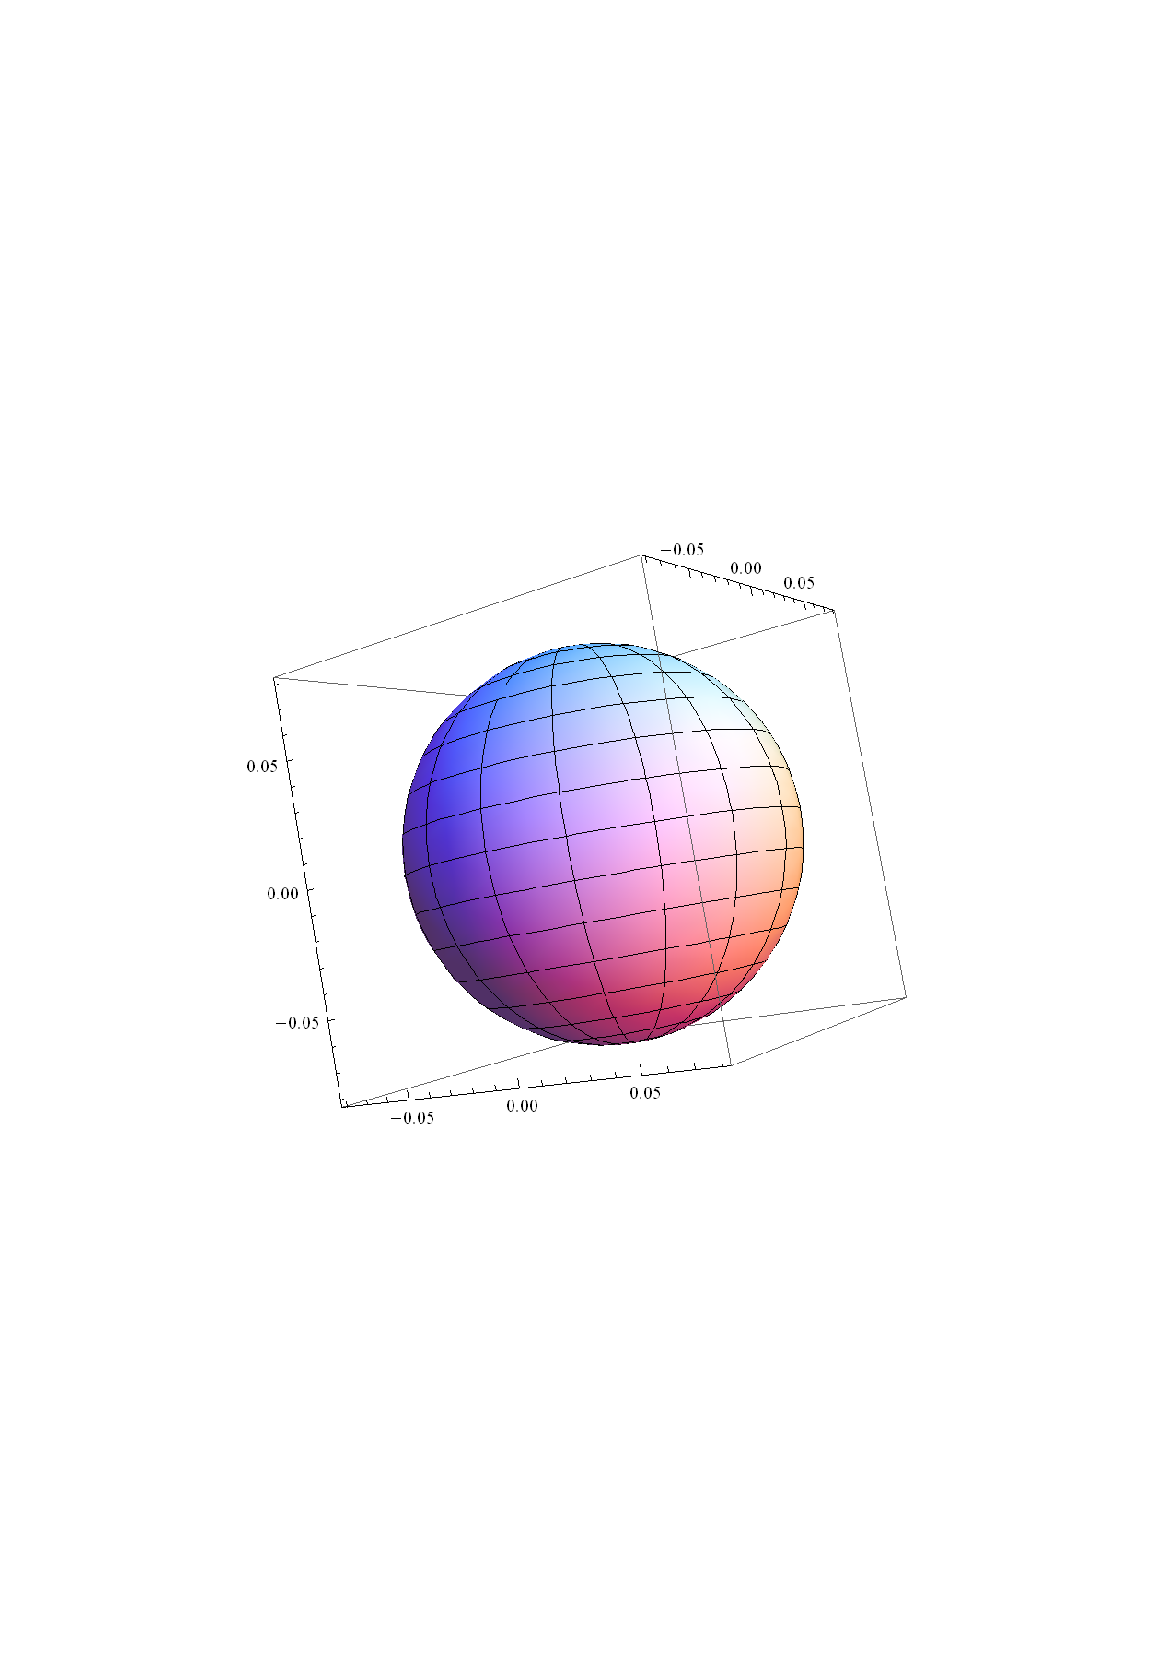
\includegraphics[width=5.722cm,height=4.842cm]{odt15-img001.emf}
  &
  [Warning: Image ignored] % Unhandled or unsupported graphics:
%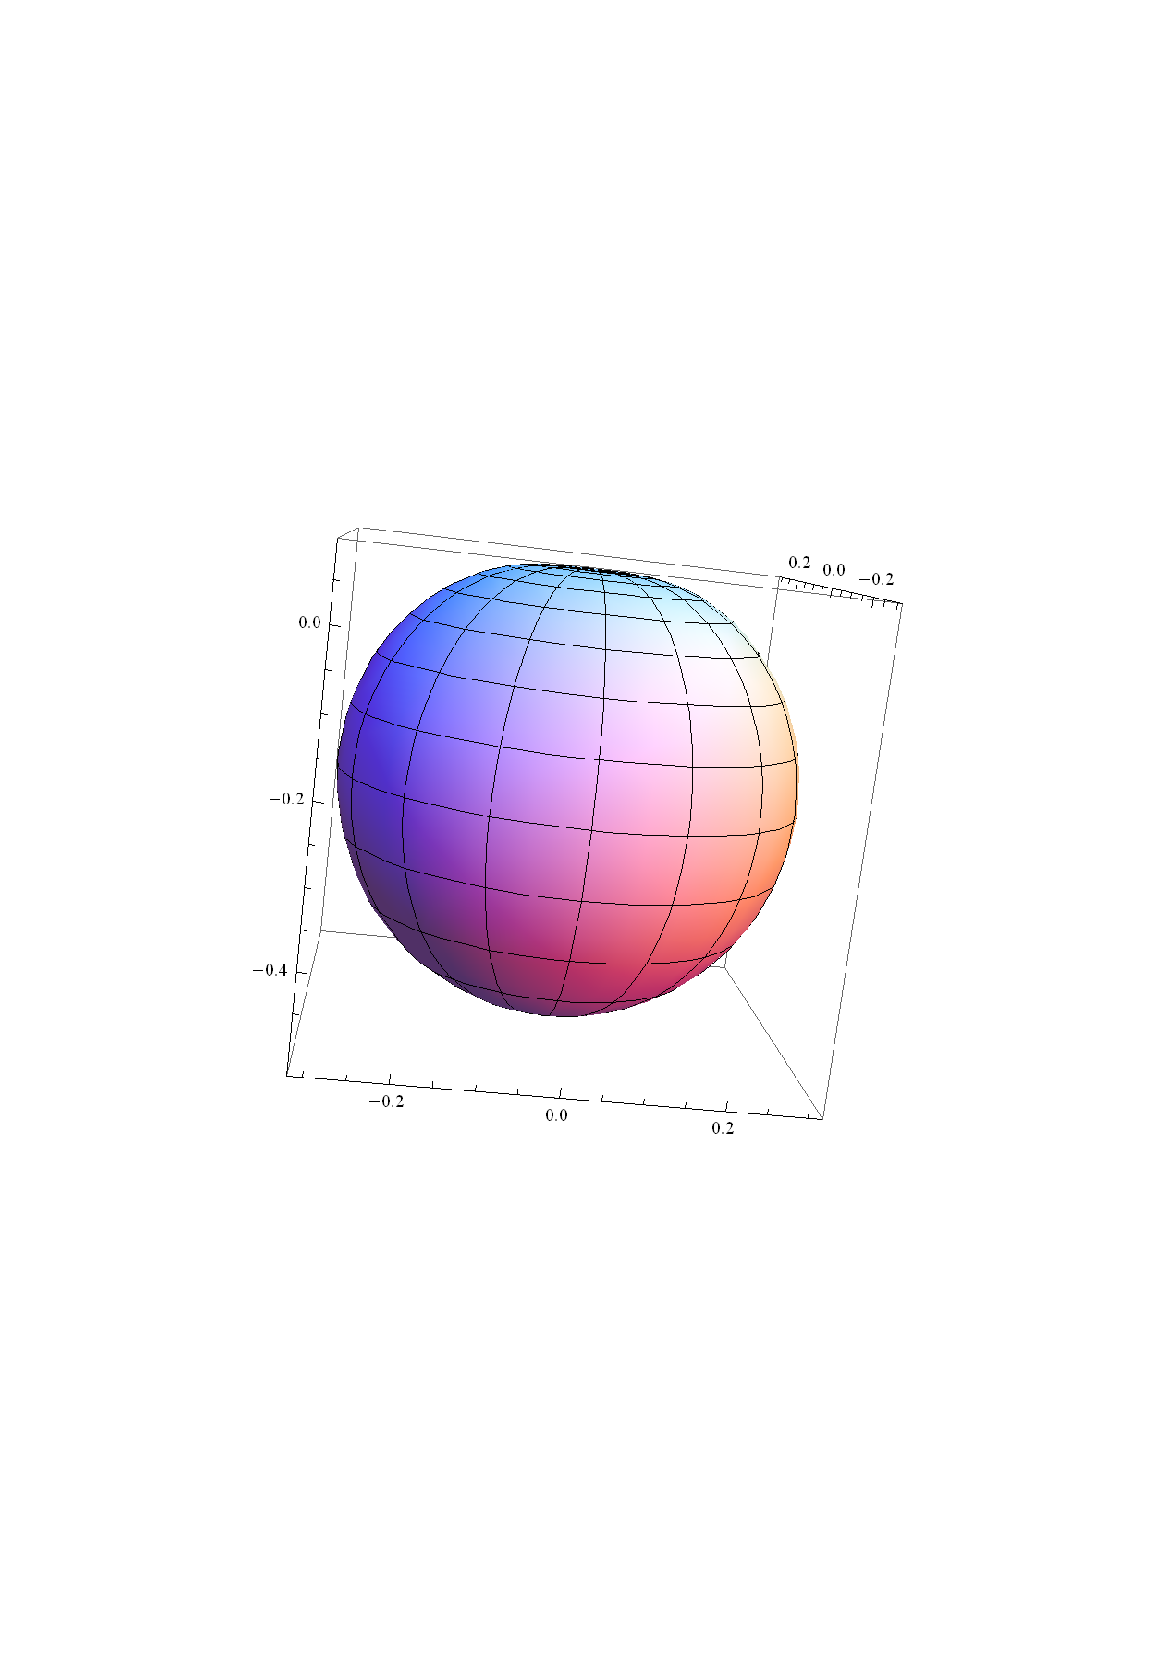
\includegraphics[width=5.106cm,height=4.748cm]{odt15-img002.emf}
 \\\hline
\foreignlanguage{english}{l = }1

\foreignlanguage{english}{m = 0} &
  [Warning: Image ignored] % Unhandled or unsupported graphics:
%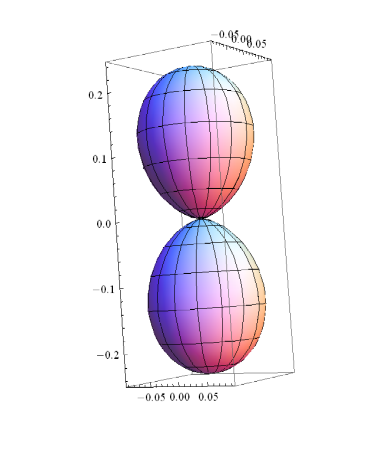
\includegraphics[width=4.948cm,height=5.9cm]{odt15-img003.emf}
  &
  [Warning: Image ignored] % Unhandled or unsupported graphics:
%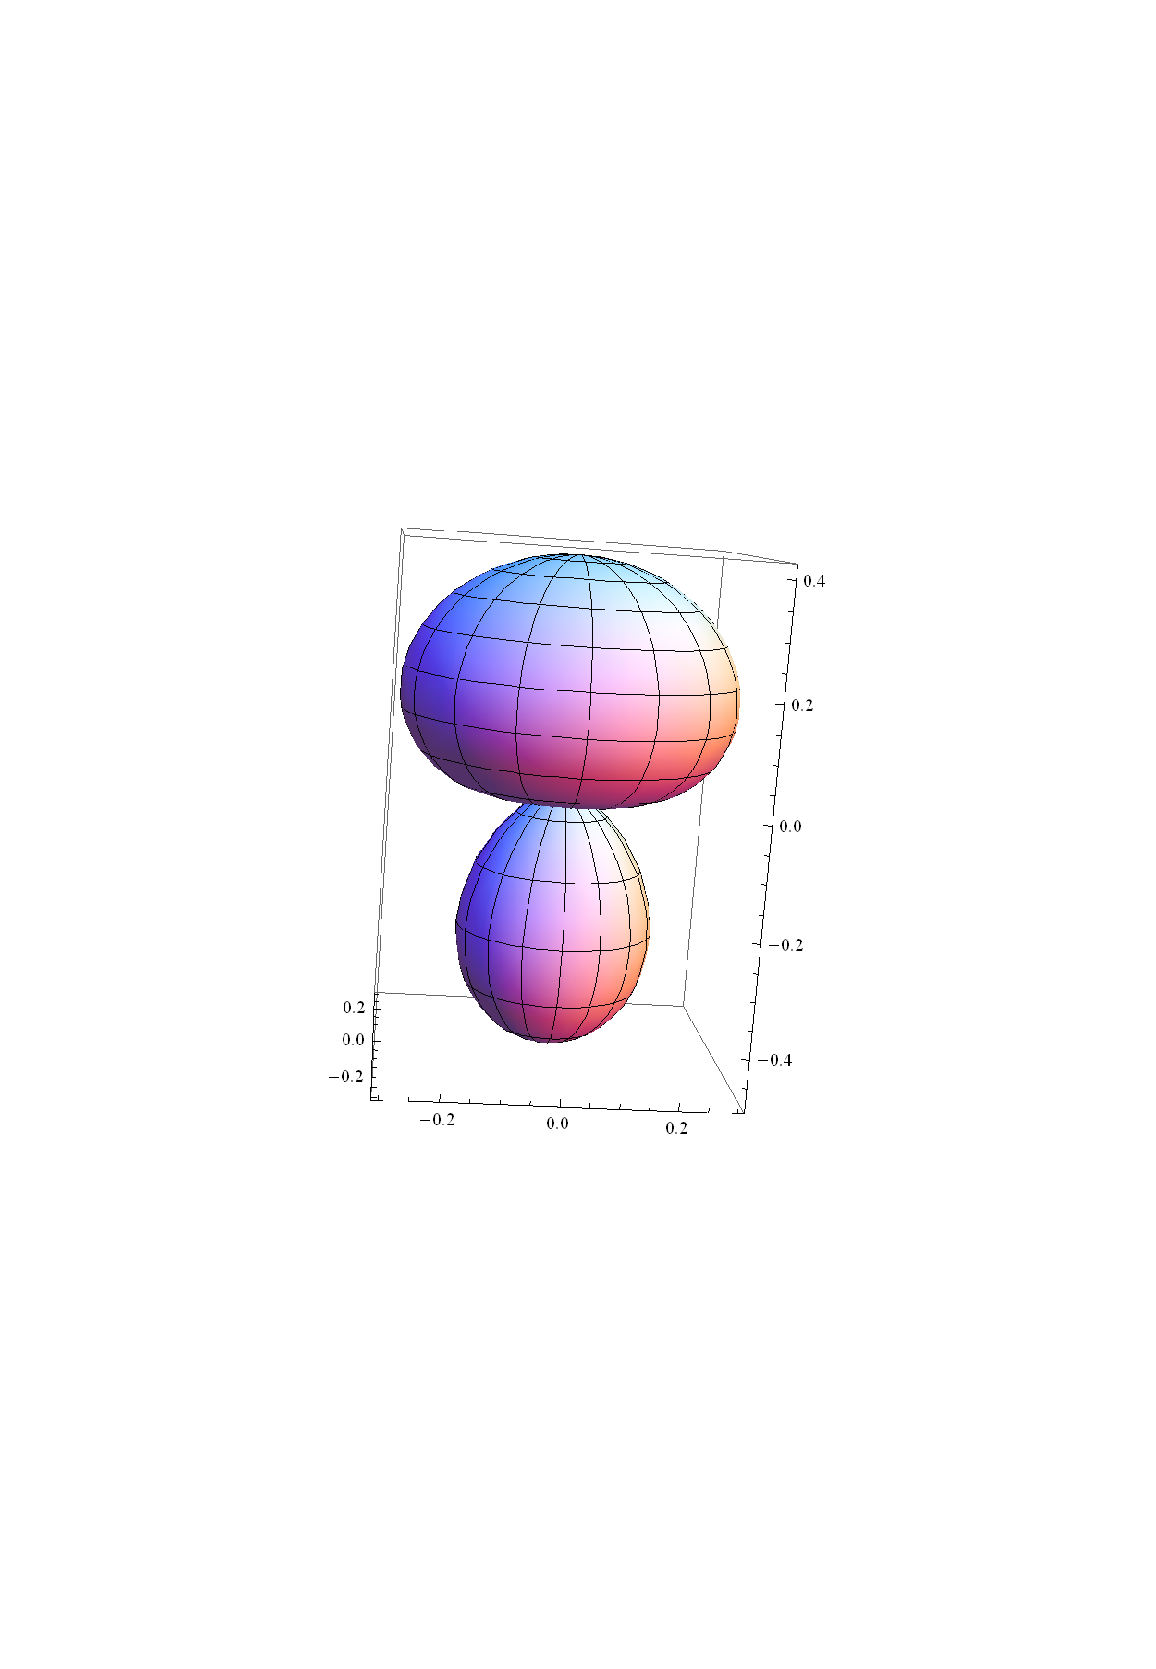
\includegraphics[width=5.027cm,height=5.457cm]{odt15-img004.emf}
 \\\hline
\foreignlanguage{english}{l = }2

\foreignlanguage{english}{m = 0} &
  [Warning: Image ignored] % Unhandled or unsupported graphics:
%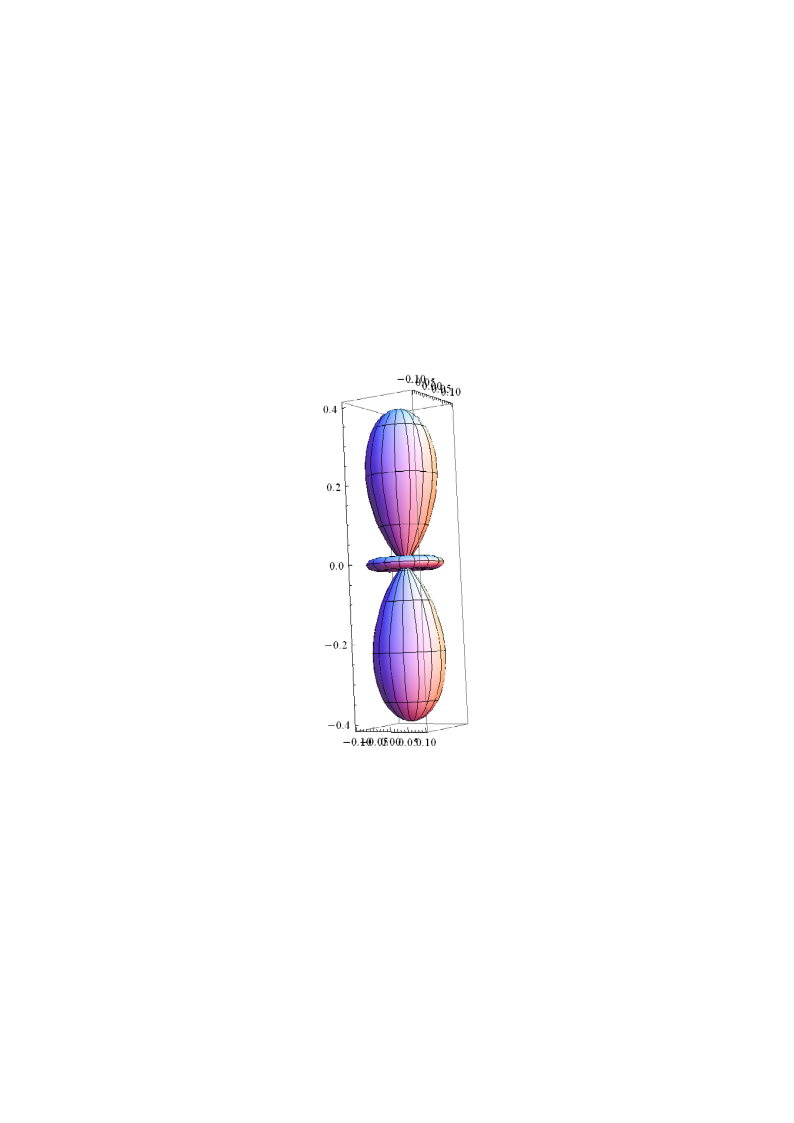
\includegraphics[width=5.292cm,height=8.44cm]{odt15-img005.emf}
  &
  [Warning: Image ignored] % Unhandled or unsupported graphics:
%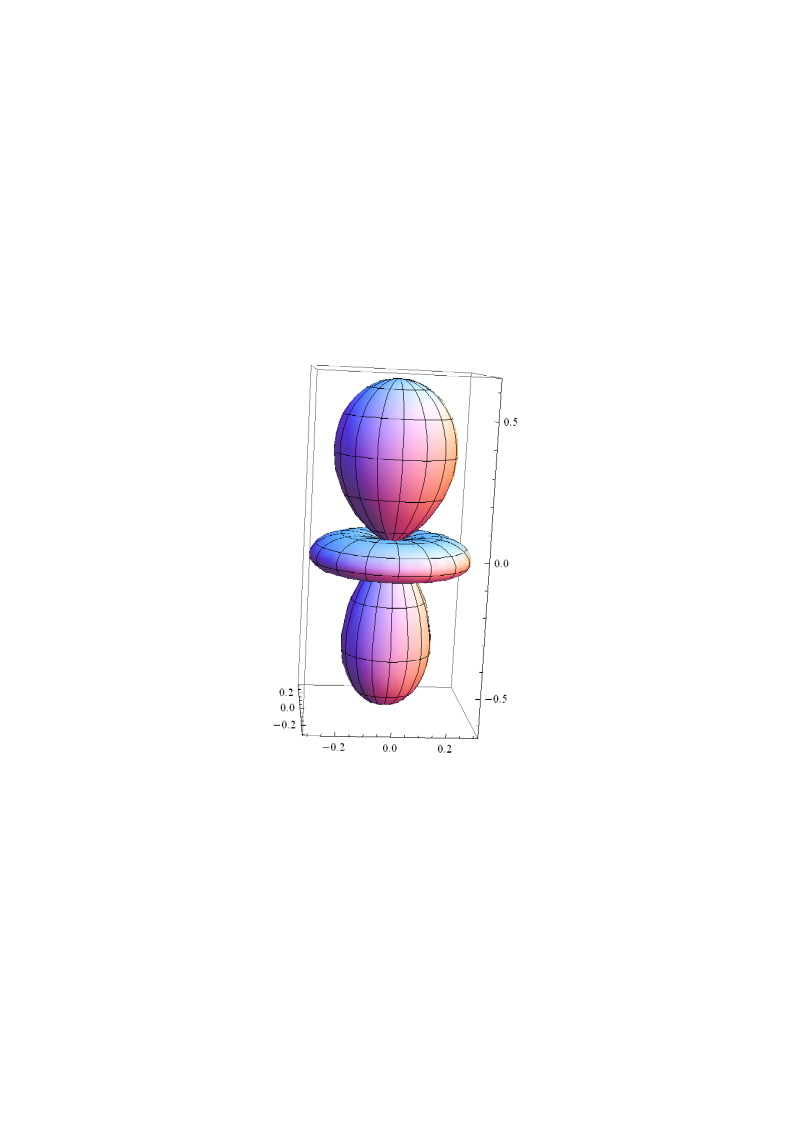
\includegraphics[width=5.136cm,height=7.646cm]{odt15-img006.emf}
 \\\hline
\foreignlanguage{english}{l = }1

\foreignlanguage{english}{m = }1 &
  [Warning: Image ignored] % Unhandled or unsupported graphics:
%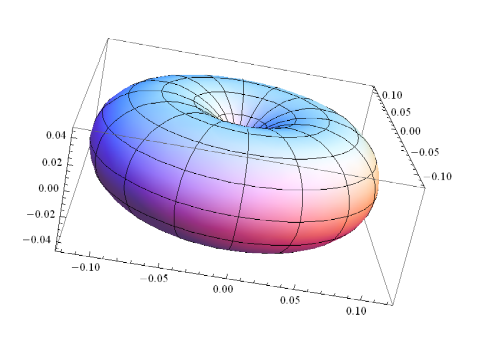
\includegraphics[width=5.72cm,height=3.731cm]{odt15-img007.emf}
  &
  [Warning: Image ignored] % Unhandled or unsupported graphics:
%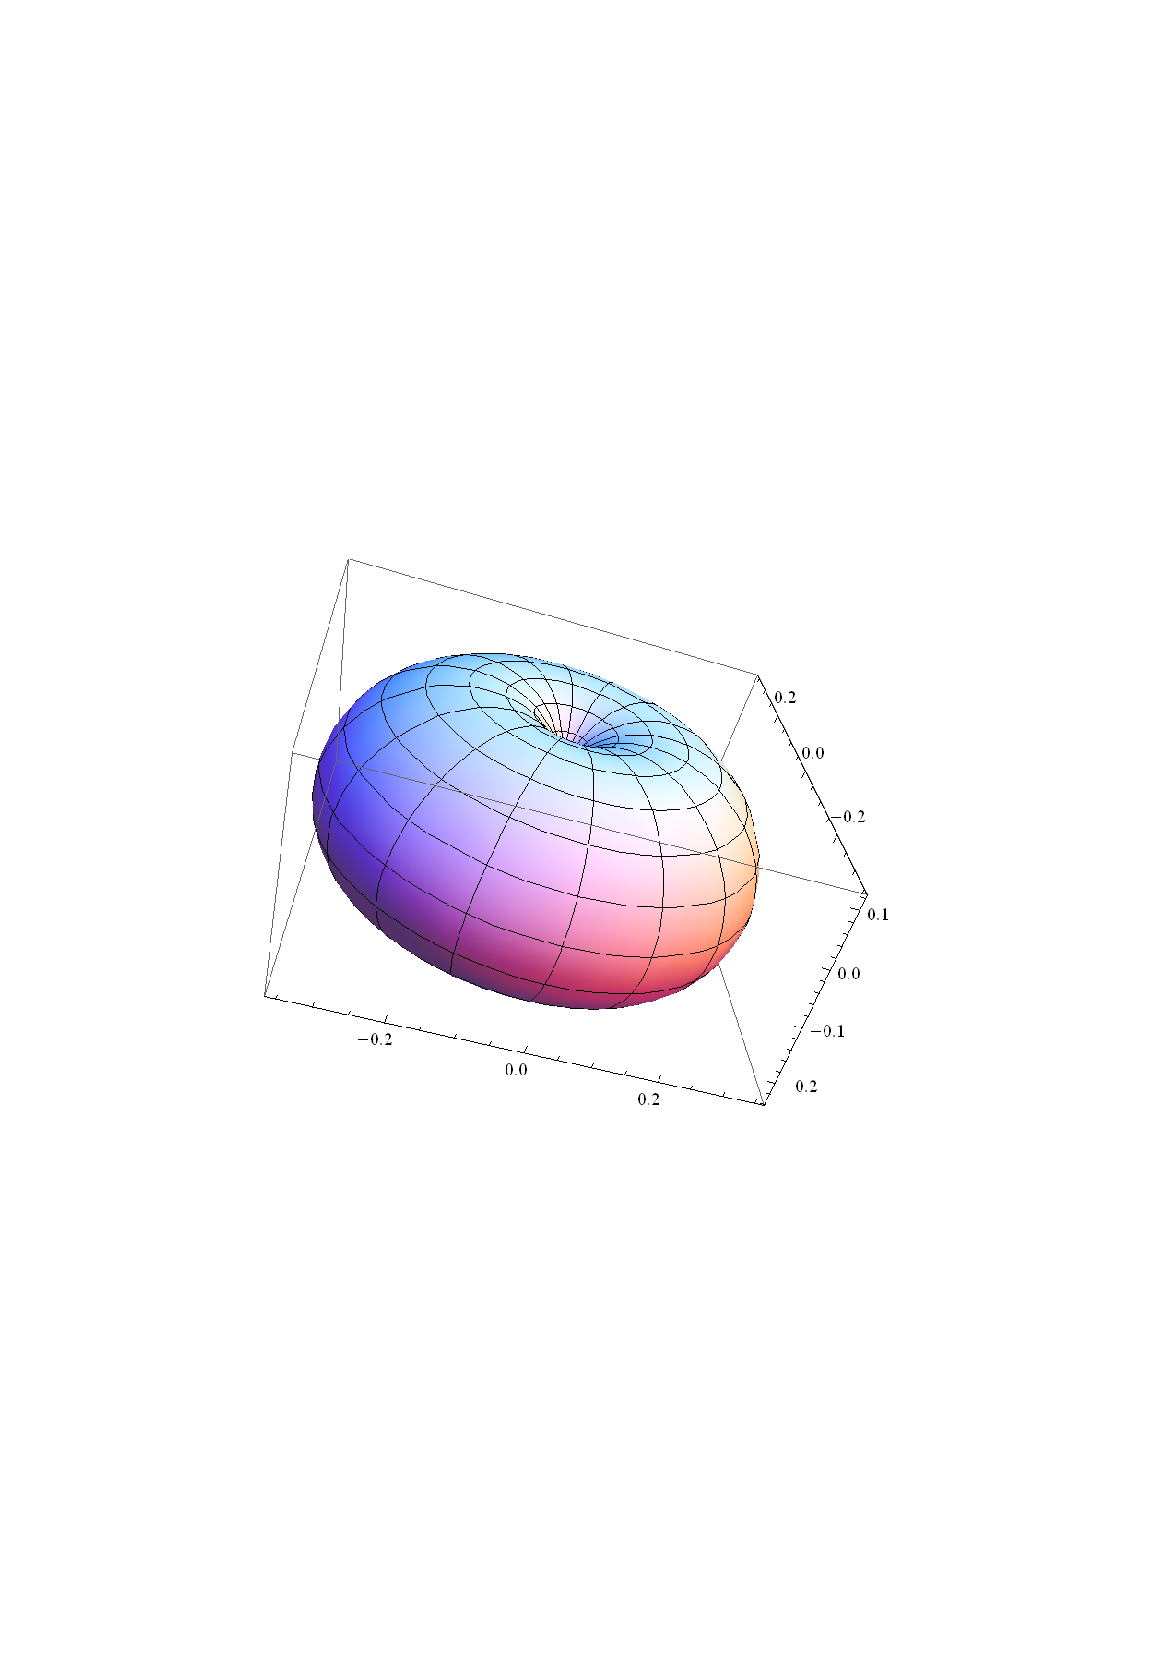
\includegraphics[width=5.099cm,height=4.26cm]{odt15-img008.emf}
 \\\hline
\foreignlanguage{english}{l = }1

\foreignlanguage{english}{m = }2 &
  [Warning: Image ignored] % Unhandled or unsupported graphics:
%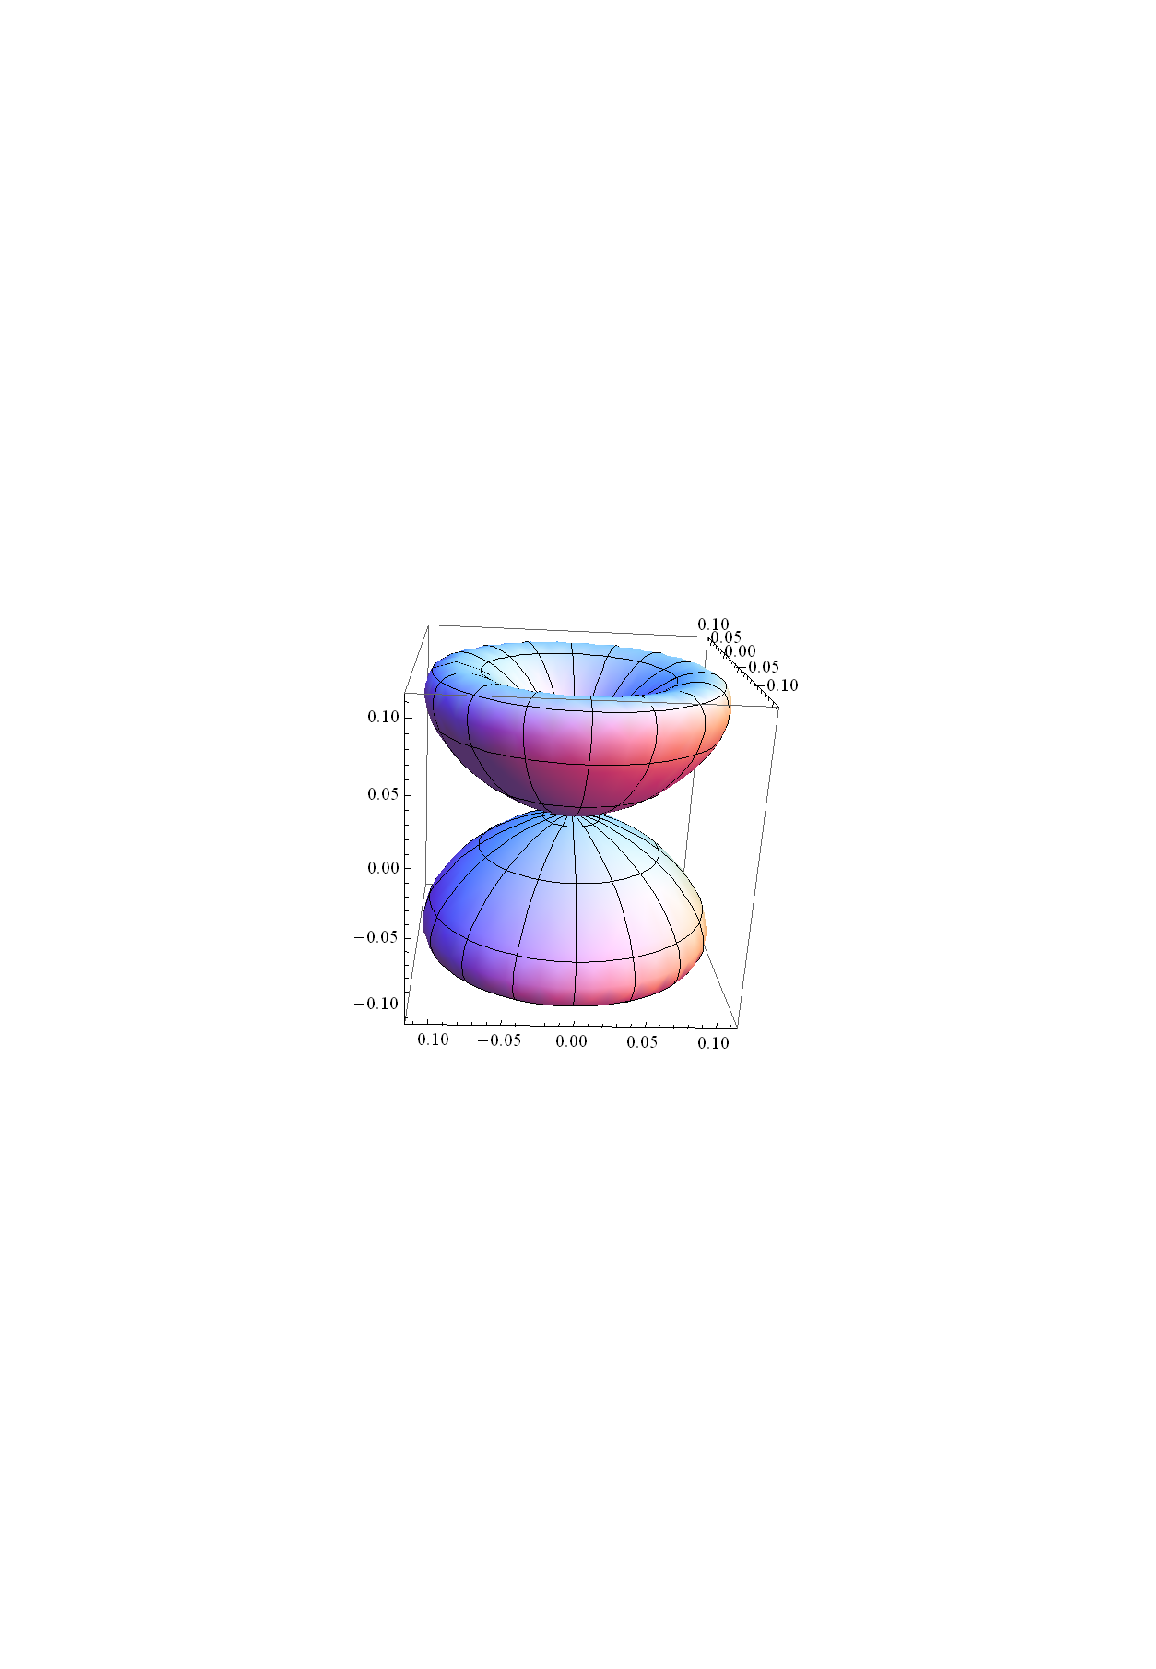
\includegraphics[width=5.292cm,height=5.078cm]{odt15-img009.emf}
  &
  [Warning: Image ignored] % Unhandled or unsupported graphics:
%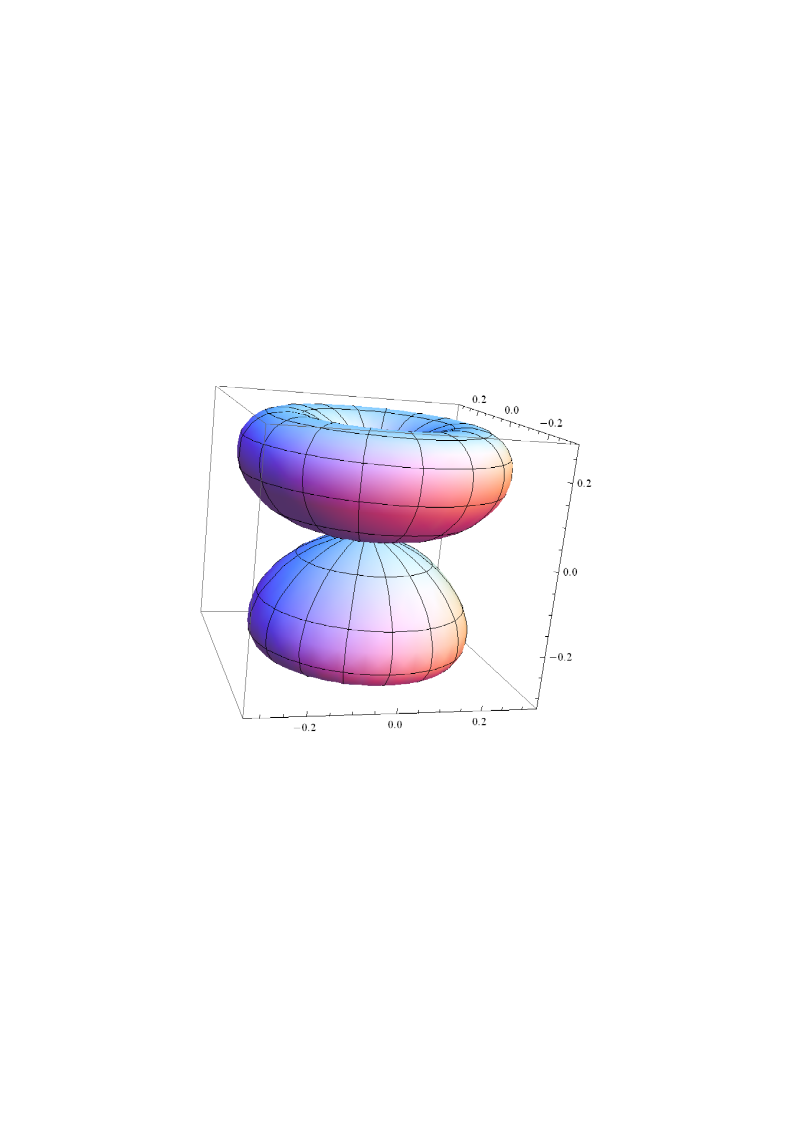
\includegraphics[width=5.98cm,height=5.017cm]{odt15-img010.emf}
 \\\hline
\foreignlanguage{english}{l = }2

\foreignlanguage{english}{m = }2 &
  [Warning: Image ignored] % Unhandled or unsupported graphics:
%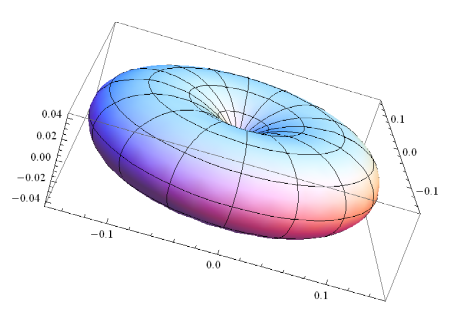
\includegraphics[width=7.541cm,height=4.916cm]{odt15-img011.emf}
  &
  [Warning: Image ignored] % Unhandled or unsupported graphics:
%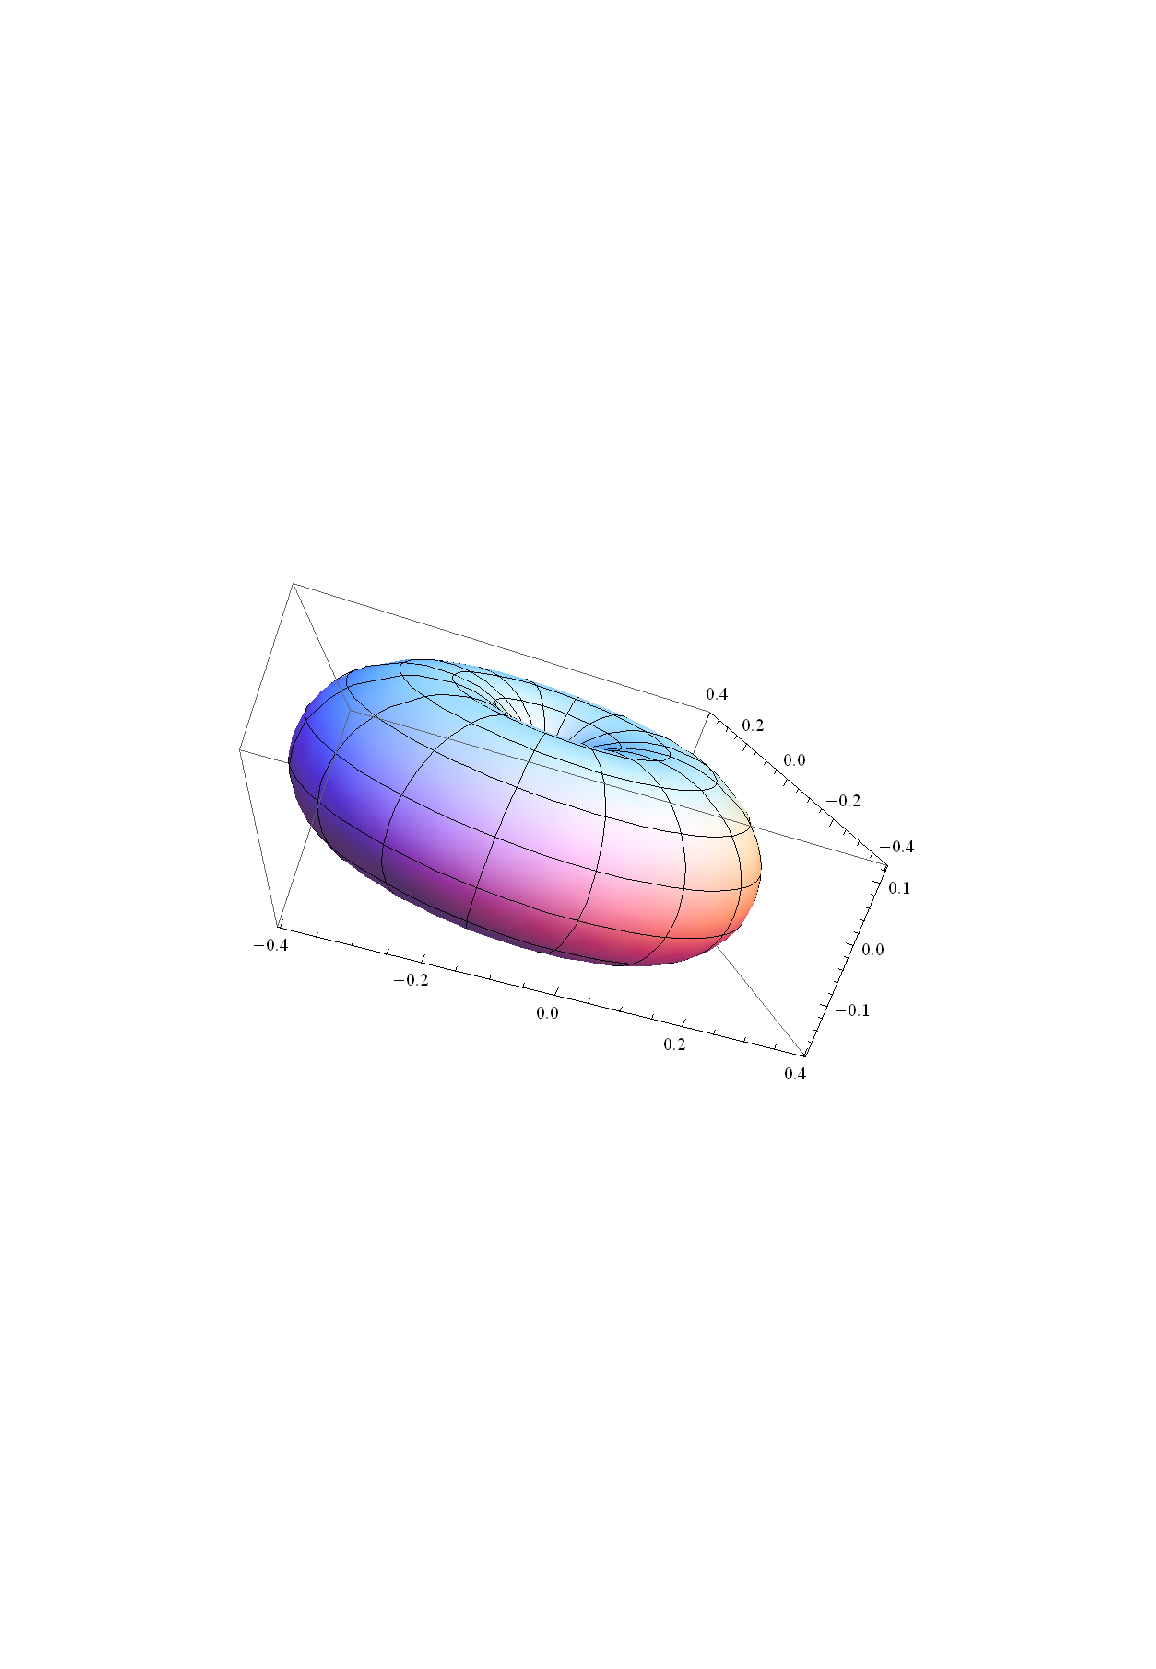
\includegraphics[width=6.773cm,height=5.48cm]{odt15-img012.emf}
 \\\hline
\end{supertabular}
\end{flushleft}

\bigskip


\bigskip

\subsubsection[1.2.2 Радиальная
часть]{1.2.2
Радиальная часть}
Т.к. уравнение на радиальную часть как в кулоновском, как и в кулон-дипольном случае можно свести к уравнению на фукцию Уитеккера, рассмотрим некоторые свойства этих функций, которые в дальнейшем будут нам полезны.

\paragraph[1.2.2.1 Свойства M{}- и W{}-
функций
Уитеккера[9{]}]{1.2.2.1
Свойства \foreignlanguage{english}{M}{}- и
\foreignlanguage{english}{W}{}- функций
Уитеккера[9]}
а) Уравнение на функции

\begin{equation*}
\frac{d^2W}{\mathit{dz}^2}+\left(\frac{-1} 4+\frac{\kappa } z+\frac{\frac 1 4-\mu ^2}{z^2}\right)W=0
\end{equation*}
б)  $z\rightarrow 0$

\begin{equation*}
M_{\kappa ,\mu }=z^{\mu +\frac 1 2}
\end{equation*}
В случае, если  $\frac 1 2-\kappa \pm \mu =-n$

\begin{equation*}
W_{\frac 1 2-\kappa \pm \mu ,\mu }=\left(-1\right)^n(1\pm 2\mu )_nz^{\frac 1 2\pm \mu }
\end{equation*}
Иначе

\begin{equation*}
W_{\kappa ,\mu }=\frac{\text{\textcyrillic{Г}}(2\mu )}{\text{\textcyrillic{Г}}\left(\frac 1 2+\mu -\kappa
\right)}z^{\frac 1 2-\mu }
\end{equation*}
в)  $z\rightarrow {\infty}$

\begin{equation*}
W_{\kappa ,\mu }\ e^{\frac{-1} 2z}z^k
\end{equation*}
В случае, если  $\mu -\kappa {\neq}-n-\frac 1 2$

\begin{equation*}
M_{\kappa ,\mu }(z){\sim}\frac{\Gamma (1+2\mu )e^{\frac 1 2z}z^{-\kappa }}{\Gamma (\frac 1 2+\mu -\kappa )}
\end{equation*}
\paragraph[1.2.2.2 Теоретический
вывод радиальной
функции]{1.2.2.2
Теоретический вывод радиальной
функции}
Рассмотрим радиальное уравнение.

\begin{equation*}
\frac 1{r^2}\frac d{\mathit{dr}}\left(r^2\frac{dR}{\mathit{dr}}\right)R+\left(\frac 2 r+2E-\frac{\lambda
}{r^2}\right)R=0(2.2.2.1)
\end{equation*}
Легко можно видеть, что по виду оно абсолютно аналогично соответствующему кулоновскому уравнению, с
заменой  $\lambda =l(l+1)$.  $\lambda $ --
собственное значение уравнения на угловую часть. Соответственно, решения будут такие же по виду.

\begin{equation*}
R=\frac 1 r\text{\textcyrillic{М}}_{\nu ,\rho }\left(r\sqrt{-8E}\right)=\frac 1
r\text{\textcyrillic{М}}_{\nu ,\rho }\left(\frac{2r}{\nu }\right)(2.2.2.2)
\end{equation*}
\begin{equation*}
E=\frac{-1}{2\nu ^2}(2.2.2.3)
\end{equation*}
\begin{equation*}
\rho _{\mathit{lm}}=\left(\lambda _{\mathit{lm}}+\frac 1 4\right)^{1/2}(2.2.2.3)
\end{equation*}
Введем понятие  $\widetilde l=\rho -\frac
1 2$ -- квазиугловой
момент.

Приведем таблицу
значений  $\widetilde l$ в
зависимости от значений дипольного момента

\begin{flushleft}
\tablefirsthead{}
\tablehead{}
\tabletail{}
\tablelasttail{}
\begin{supertabular}{|m{2.158cm}|m{2.292cm}|m{2.109cm}|m{2.112cm}|m{2.382cm}|m{2.111cm}|m{2.162cm}|}
\hline
\centering \textit{\textcolor{black}{d}} &
\multicolumn{3}{m{6.913cm}|}{\centering \textit{\textcolor{black}{m = 0}}} &
\multicolumn{2}{m{4.6930003cm}|}{\centering \textit{\textcolor{black}{m = 1}}} &
\textit{\textcolor{black}{m = 2}}\\\hline
 &
\centering \textit{\textcolor{black}{l = 0}} &
\centering \textit{\textcolor{black}{l = 1}} &
\centering \textit{\textcolor{black}{l = 2}} &
\centering \textit{\textcolor{black}{l = 1}} &
\centering \textit{\textcolor{black}{l = 2}} &
\centering\arraybslash \textit{\textcolor{black}{l = 2}}\\\hline
\raggedleft \textcolor{black}{0,2} &
\raggedleft \textcolor{black}{{}-0,02715} &
\raggedleft \textcolor{black}{1,00524} &
\raggedleft \textcolor{black}{2,00076} &
\raggedleft \textcolor{black}{0,997334} &
\raggedleft \textcolor{black}{2,00038} &
\raggedleft\arraybslash \textcolor{black}{1,99924}\\\hline
\raggedleft \textcolor{black}{0,4} &
\raggedleft \textcolor{black}{{}-0,11636} &
\raggedleft \textcolor{black}{1,01989} &
\raggedleft \textcolor{black}{2,00306} &
\raggedleft \textcolor{black}{0,989341} &
\raggedleft \textcolor{black}{2,0015} &
\raggedleft\arraybslash \textcolor{black}{1,99695}\\\hline
\raggedleft \textcolor{black}{0,6} &
\raggedleft \textcolor{black}{{}-0,33328} &
\raggedleft \textcolor{black}{1,04134} &
\raggedleft \textcolor{black}{2,00694} &
\raggedleft \textcolor{black}{0,976038} &
\raggedleft \textcolor{black}{2,00329} &
\raggedleft\arraybslash \textcolor{black}{1,99315}\\\hline
\raggedleft \textcolor{black}{0,8} &
\textcolor{black}{{}-} &
\raggedleft \textcolor{black}{1,06655} &
\raggedleft \textcolor{black}{2,01244} &
\raggedleft \textcolor{black}{0,957442} &
\raggedleft \textcolor{black}{2,00567} &
\raggedleft\arraybslash \textcolor{black}{1,98783}\\\hline
\raggedleft \textcolor{black}{1,0} &
\textcolor{black}{{}-} &
\raggedleft \textcolor{black}{1,09285} &
\raggedleft \textcolor{black}{2,01961} &
\raggedleft \textcolor{black}{0,933563} &
\raggedleft \textcolor{black}{2,00851} &
\raggedleft\arraybslash \textcolor{black}{1,98101}\\\hline
\raggedleft \textcolor{black}{1,2} &
\textcolor{black}{{}-} &
\raggedleft \textcolor{black}{1,11824} &
\raggedleft \textcolor{black}{2,02852} &
\raggedleft \textcolor{black}{0,904393} &
\raggedleft \textcolor{black}{2,01168} &
\raggedleft\arraybslash \textcolor{black}{1,97268}\\\hline
\raggedleft \textcolor{black}{1,4} &
\textcolor{black}{{}-} &
\raggedleft \textcolor{black}{1,1413} &
\raggedleft \textcolor{black}{2,03918} &
\raggedleft \textcolor{black}{0,869881} &
\raggedleft \textcolor{black}{2,01501} &
\raggedleft\arraybslash \textcolor{black}{1,96287}\\\hline
\raggedleft \textcolor{black}{1,6} &
\textcolor{black}{{}-} &
\raggedleft \textcolor{black}{1,16111} &
\raggedleft \textcolor{black}{2,05158} &
\raggedleft \textcolor{black}{0,829924} &
\raggedleft \textcolor{black}{2,01835} &
\raggedleft\arraybslash \textcolor{black}{1,95158}\\\hline
\raggedleft \textcolor{black}{1,8} &
\textcolor{black}{{}-} &
\raggedleft \textcolor{black}{1,17709} &
\raggedleft \textcolor{black}{2,06566} &
\raggedleft \textcolor{black}{0,784337} &
\raggedleft \textcolor{black}{2,02156} &
\raggedleft\arraybslash \textcolor{black}{1,93883}\\\hline
\raggedleft \textcolor{black}{2,0} &
\textcolor{black}{{}-} &
\raggedleft \textcolor{black}{1,1889} &
\raggedleft \textcolor{black}{2,08132} &
\raggedleft \textcolor{black}{0,732823} &
\raggedleft \textcolor{black}{2,02448} &
\raggedleft\arraybslash \textcolor{black}{1,92462}\\\hline
\end{supertabular}
\end{flushleft}
{\centering
Таблица 1.
\par}

Для того, чтобы выполнялись граничные условия
при  $r\rightarrow {\infty}$, необходимо,
чтобы между  $\rho $ и  $\nu $
выполнялось соотношение (см. свойство (в) п. 1.2.2.1).

\begin{equation*}
\nu =n_r+\rho +\frac 1 2(2.2.2.4)
\end{equation*}
Учитывая, что  $n=n_r+l+1$,  $\nu =n+\widetilde
l-l$

Для квантового дефекта тогда получим выражение
$\delta =l+\frac 1 2-\rho $

При использовании исключительно теоретических построений возникает следующая проблема: рассчитанные квантовые дефекты включают в себя только дипольную часть и не учитывают короткодействующую часть потенциала.

\begin{equation*}
\delta _{\mathit{calc}}{\neq}\delta _{\mathit{obs}}\rightarrow E_{\mathit{calc}}{\neq}E_{\mathit{obs}}
\end{equation*}
\paragraph[1.2.2.3 Модельный
потенциал
Саймонса ]{1.2.2.3
Модельный потенциал
Саймонса }

Эмпирически наблюдаемый квантовый дефект можно учесть, рассматривая модельный потенциал
следующего вида[10]:

\begin{equation*}
V\left(r\right)=\frac{\lambda \left(\lambda +1\right)-\widetilde l(\widetilde l+1)}{2r^2}-\frac 1 r(2.2.3.1)
\end{equation*}
 $\lambda $\textit{ - }параметр,
определяемый эмпирически.

Вводя замену  $R(r)=\frac{\mu (r)} r$,
получаем
уравнение на  $\mu (r)$

\begin{equation*}
\frac{-1} 2\frac{d^2\mu }{\mathit{dr}^2}+\left[\frac{\lambda (\lambda +1)}{2r^2}-\frac 1 r\right]\mu =E\mu (2.2.3.2)
\end{equation*}
Уравнение
имеет\foreignlanguage{english}{
}следующее решение

\begin{equation*}
\mu \left(r\right)=\text{\textcyrillic{М}}_{\frac 1{\sqrt{-2E}},\lambda +\frac 1
2}\left(r\sqrt{-8E}\right)(2.2.3.3)
\end{equation*}
Энергия в этом выражении -- величина, определяемая экспериментально.

Можно воспользоваться известной формулой

\begin{equation*}
E=\frac{-1}{2(n-\delta )^2}
\end{equation*}
Тогда чтобы обеспечить
сходимость  $\text{\textcyrillic{М}}$ --
функции Уитеккера на бесконечности,

\begin{equation*}
\lambda =l-\delta +K(2.2.3.4)
\end{equation*}
 $K$\textit{ -- }целое число

Обсудим более подробно проблему
выбора \foreignlanguage{english}{K}.

Т.к. при малых \foreignlanguage{english}{\textit{r}}
центростремительный
член  $\frac{l(l+1)}{2r^2}$
преобладает в
\foreignlanguage{english}{\textit{V}}\textit{(}\foreignlanguage{english}{\textit{r}}\textit{)},
Саймонс в оригинальной
статье [10, стр. 646]
предлагает
определить \foreignlanguage{english}{\textit{K}}
таким образом,
чтобы  $| \lambda -l| $ был
минимальным.

Тогда  $k=\mathit{Round}(\delta )$

 $\mathit{Round}\left(\delta \right)$\textit{ -- }ближайшее
к  $\delta $ целое число.

В статье 1995 года [11, стр.
311] Мартин, довольно
подробно обсуждая
проблему выбора  $k$,
указывает на то, что количество узлов радиальной
функции равно  $n-l-k-1$.

С математической точки зрения допустимы следующие
значения \foreignlanguage{english}{\textit{k}}

\begin{equation*}
\delta -l-\frac 3 2<k{\leq}n-l-1
\end{equation*}
В качестве возможного выбора
Мартин приводит  $k=0$. В
этом случае количество узлов в волновой функции такое же, как у соответствующей волновой функции атома водорода.

В собственной работе Мартин
использует  $c=2-l$ для  $l=0,1,2$.
В этом случае радиальная волновая функция
при  $n=l$ не имеет узлов.

В статье 2002 года [12, стр.75]
Алчеев, также обсуждая проблему
выбора \foreignlanguage{english}{k},
использует для него следующее выражение.

\begin{equation*}
\lambda =n-\delta -k-1
\end{equation*}
Алчеев определяет  $k$
таким образом:

\begin{equation*}
k=n-n_{\mathit{cl}}(2.2.3.5)
\end{equation*}
 $n_{\mathit{cl}}$\textit{ -- }количество
заполненных электронных оболочек.

Можно сделать вывод, что рассмотренные авторы определяют
параметр \foreignlanguage{english}{k}
существенно по-разному, хотя результат расчета радиального матричного элемента может сильно зависеть от этого параметра.

\paragraph[1.2.2.4 Метод
Бейтс{}-Дамгард ]{1.2.2.4
Метод
Бейтс-Дамгард }
В методе, предложенном в статье Бейтса-Дамгард 1949
года [13], потенциал
заменяется на

\begin{equation*}
V=\frac 1 r
\end{equation*}
При этом энергия, входящая в уравнение, не является его собственным значением, а является экспериментально измеренной величиной.

\begin{equation*}
\frac{d^2R}{\mathit{dr}^2}+\left(\frac 2 r-\frac{l(l+1)}{r^2}-E\right)R=0
\end{equation*}
 $E$ -- энергия,
измеренная экспериментальным образом

Решение должно удовлетворять граничным
условиям  $R\rightarrow 0$ при $r\rightarrow {\infty}$

Т.к.  $E$ - не собственное
значение дифференциального уравнения, решение будет расходиться
при  $r\rightarrow 0$.

Для нас наиболее подходящим будет решение

\begin{equation*}
R=W_{\nu _{\mathit{klm}},l+\frac 1 2}\left(\frac{2r}{\nu _{\mathit{klm}}}\right)(2.2.4.1)
\end{equation*}
При этом нормировочный фактор будет:

\begin{equation*}
N=\frac 1{\sqrt{\nu _{\mathit{klm}}\text{\textcyrillic{Г}}(\nu
_{\mathit{klm}}+l-1)\text{\textcyrillic{Г}}(\nu _{\mathit{klm}}-l)}}(2.2.4.2)
\end{equation*}
В наших расчетах  $l\rightarrow
\widetilde l$.

Конечный вид радиальной части будет следующим:

\begin{equation*}
R=\left(1+\frac{d\delta _{\mathit{lm}}}{d\nu _{\mathit{klm}}}\right)^{-1/2}\left(\nu
_{\mathit{klm}}\text{\textcyrillic{Г}}(\nu _{\mathit{klm}}+\widetilde l-1)\text{\textcyrillic{Г}}(\nu
_{\mathit{klm}}-\widetilde l)\right)^{-1/2}W_{\nu _{\mathit{klm}},\widetilde l+\frac 1 2}\left(\frac{2r}{\nu
_{\mathit{klm}}}\right)(2.2.4.3)
\end{equation*}
Нормировочный фактор  $\left(1+\frac{d\delta _{\mathit{lm}}}{d\nu _{\mathit{klm}}}\right)^{-1/2}$
был предложен и выведен Ситоном  в статье 1958 [14].

Рассмотрим отдельно проблему с невыполнением граничных условий (при  $r\rightarrow 0,R\rightarrow \mathit{ComplexInfinity}$)

Данную проблему можно решить путем введения эффективного радиуса, который представляет собой классическую точку поворота [15].
\begin{equation*}
 \frac{\lambda }{r^2}-\frac 2 r=\frac{-1}{\nu _{\mathit{klm}}^2}
\end{equation*}
\begin{equation*}
 \frac{r^2}{\nu _{\mathit{klm}}^2}-2r+\lambda =0
\end{equation*}
\begin{equation*}
 r_c=\left(1-\sqrt{1-\frac{\widetilde l(\widetilde l+1)}{\nu _{\mathit{klm}}^2}}\right)\nu
_{\mathit{klm}}^2(2.2.4.4)
\end{equation*}

\bigskip

\textbf{Сводная таблица (для радиальной части)}

\begin{equation*}
R=W_{\nu ,\rho }\left(\frac{2r}{\nu }\right)
\end{equation*}
\begin{flushleft}
\tablefirsthead{}
\tablehead{}
\tabletail{}
\tablelasttail{}
\begin{supertabular}{|m{2.723cm}|m{2.61cm}|m{3.931cm}|m{3.155cm}|m{3.222cm}|}
\hline
~
 &
 $\nu $ &
 $\rho $ &
\textbf{Особенности} &
\centering\arraybslash \textbf{Нижний
предел
интегрирования}\\\hline
\textbf{Модельный
потенциал
Саймонса} &
 $\nu _{\mathit{obs}}$ &
 $l-n+\nu _{\mathit{obs}}+K+\frac 1 2$ &
Нужно подбирать
\foreignlanguage{english}{k} &
\textbf{0}\\\hline
\textbf{Метод
Бейтса-Дамгаард} &
 $\nu _{\mathit{obs}}$ &
 $\widetilde l_{\mathit{lm}}+\frac 1 2$ &
Расходится в 0 &
 $\left(1-\sqrt{1-\frac{\widetilde l(\widetilde l+1)}{\nu _{\mathit{klm}}^2}}\right)\nu _{\mathit{klm}}^2$\\\hline
\end{supertabular}
\end{flushleft}
{\centering
\textbf{Таблица 2.}
\par}


\bigskip

\textbf{Сравнение
графиков (нормированных) радиальных функций, построенных различными
способами}

\textbf{(}\foreignlanguage{english}{\textbf{NaHe}}\textbf{, }\foreignlanguage{english}{\textbf{n}}\textbf{ = 3,
}\foreignlanguage{english}{\textbf{l}}\textbf{ = 1, }\foreignlanguage{english}{\textbf{m}}\textbf{ = 0)}

  [Warning: Image ignored] % Unhandled or unsupported graphics:
%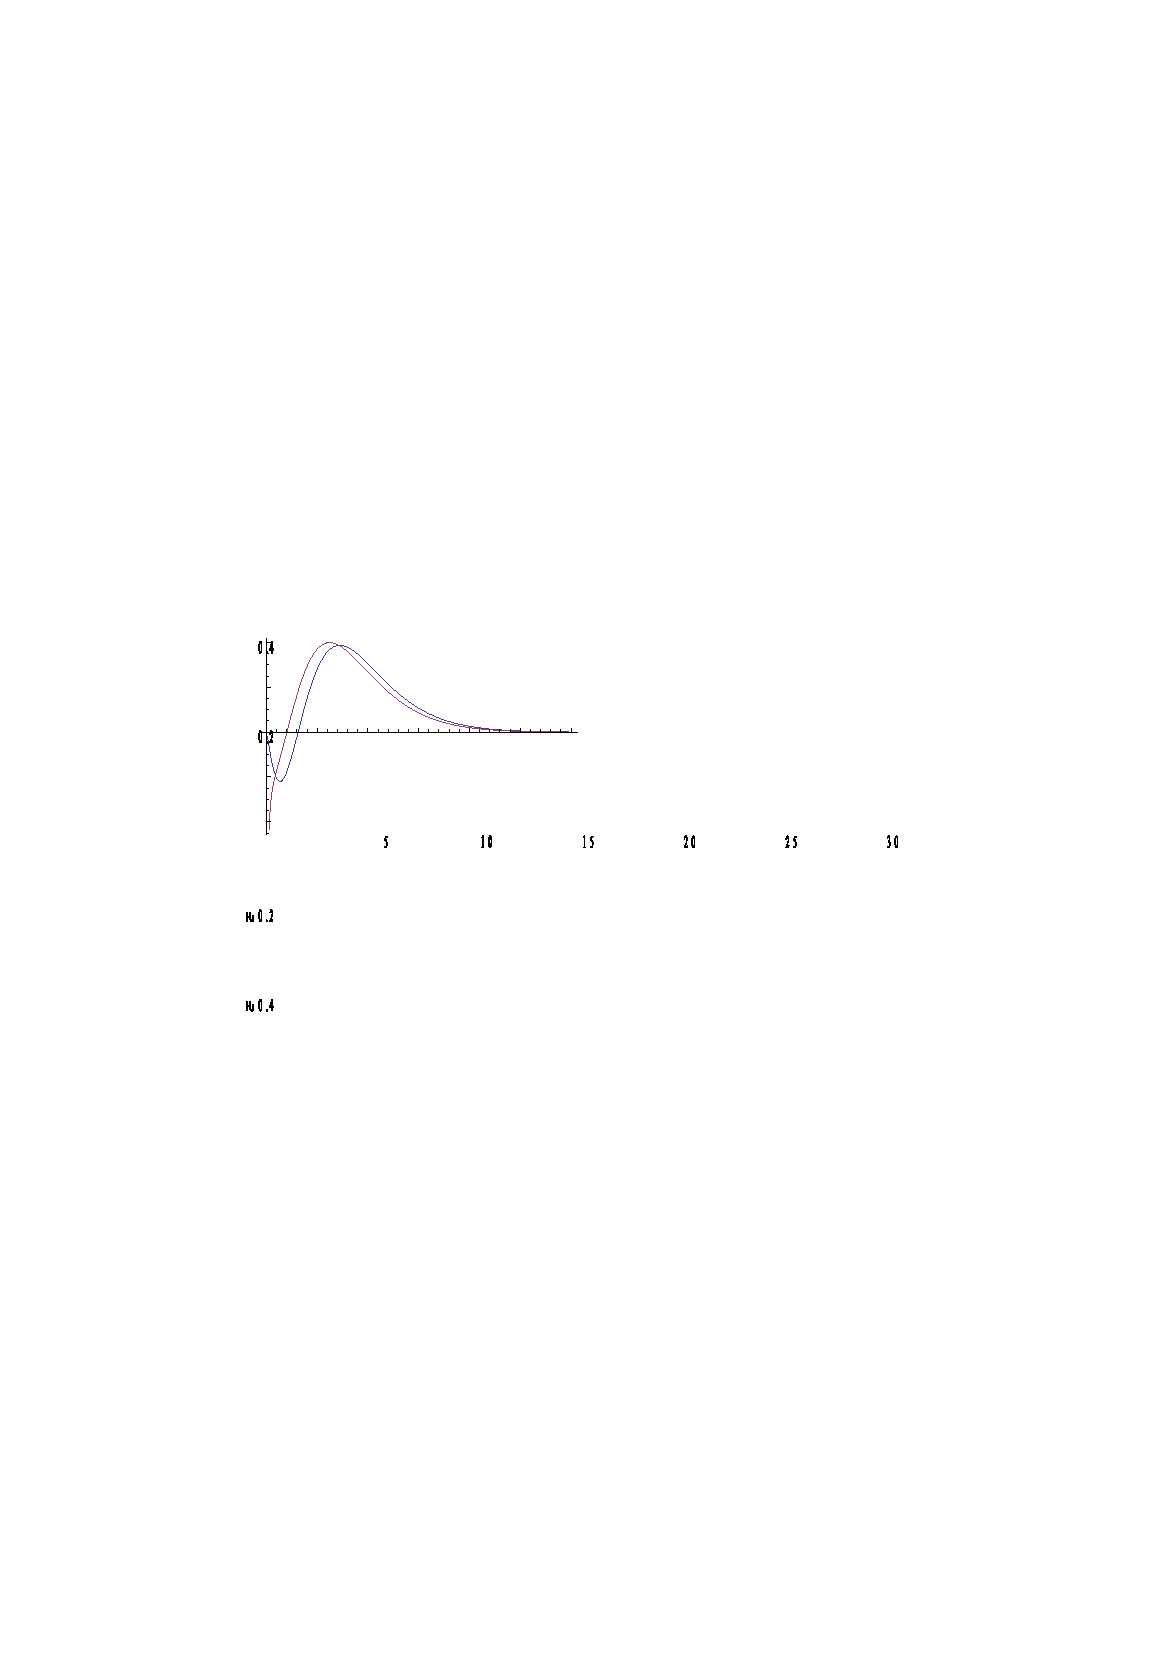
\includegraphics[width=9.537cm,height=5.655cm]{odt15-img014.emf}


\begin{flushleft}
\tablefirsthead{}
\tablehead{}
\tabletail{}
\tablelasttail{}
\begin{supertabular}{m{3.741cm}m{12.927cm}}
[Warning: Draw object ignored] &
Модельный потенциал
Саймонса\\
{}[Warning: Draw object ignored] &
Метод
Бейтса-Дамгард\\
\end{supertabular}
\end{flushleft}

\bigskip

\textbf{(}\foreignlanguage{english}{\textbf{NaHe}}\textbf{, }\foreignlanguage{english}{\textbf{n}}\textbf{ = 3,
}\foreignlanguage{english}{\textbf{l}}\textbf{ = }\foreignlanguage{english}{\textbf{0}}\textbf{,
}\foreignlanguage{english}{\textbf{m}}\textbf{ = 0)}

  [Warning: Image ignored] % Unhandled or unsupported graphics:
%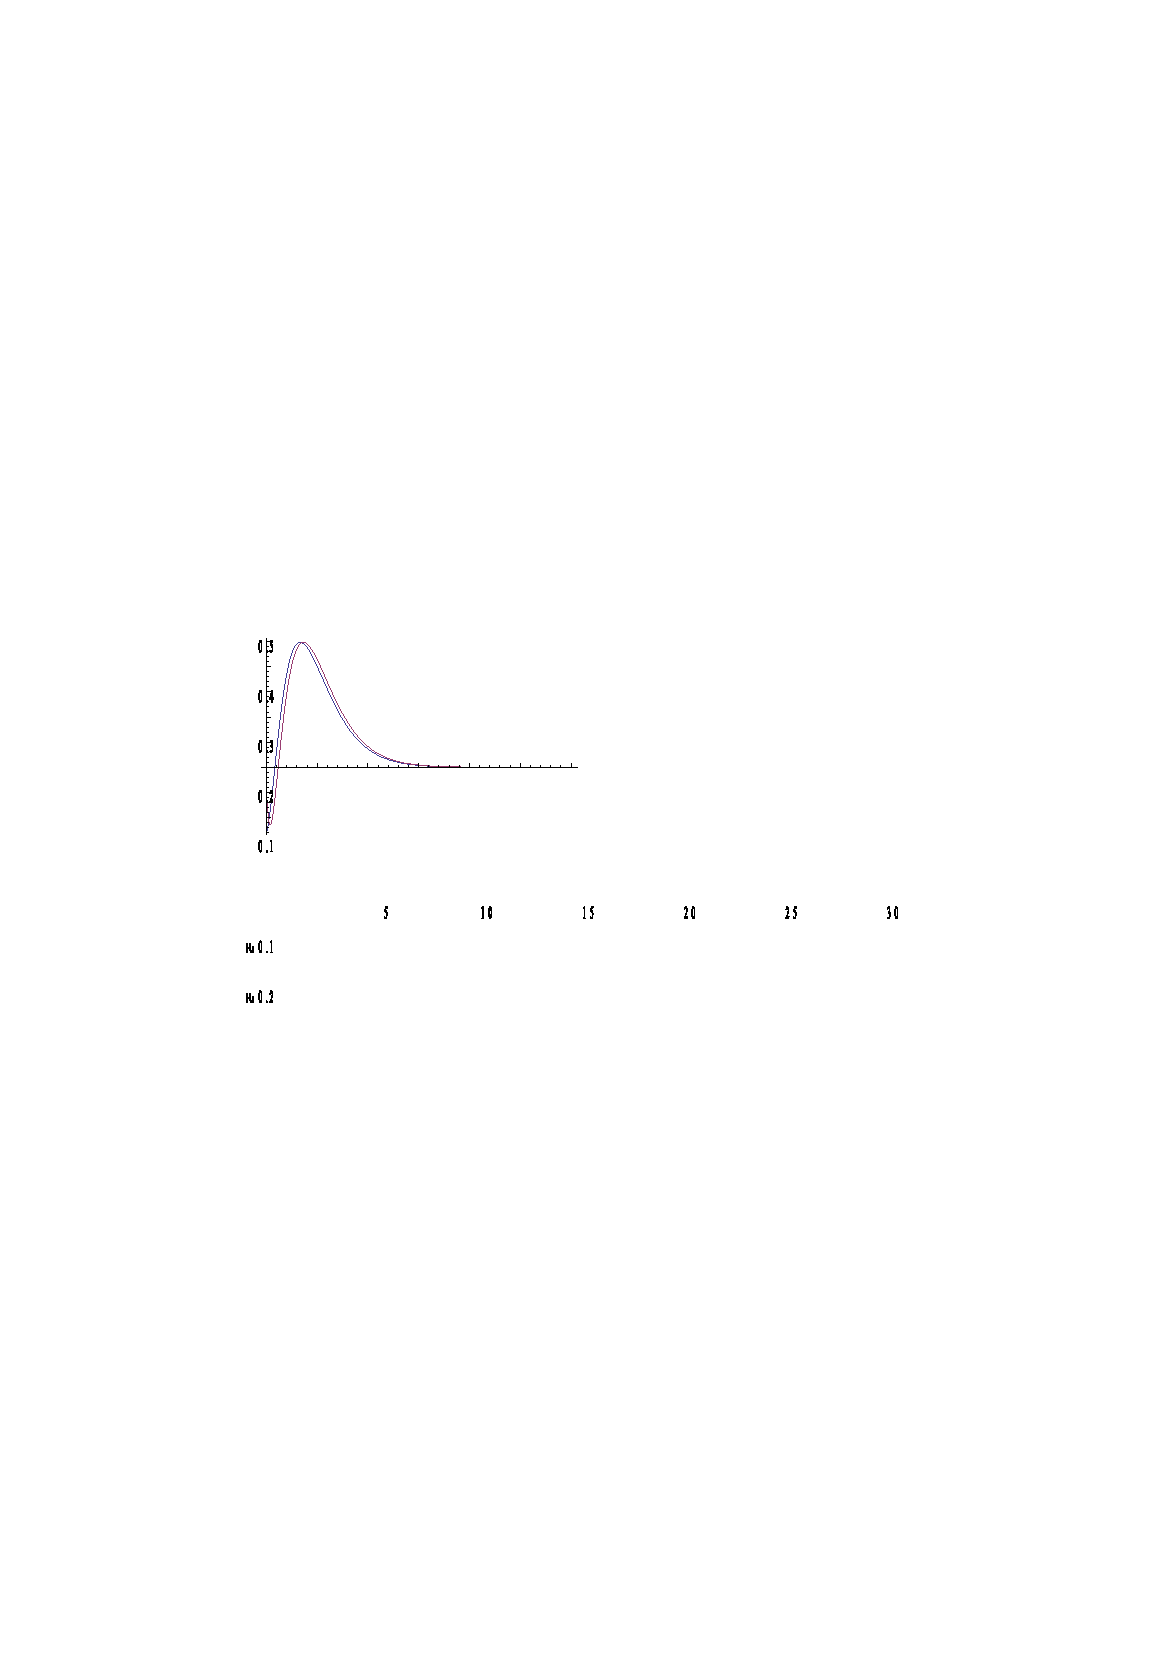
\includegraphics[width=11.592cm,height=6.904cm]{odt15-img015.emf}


\begin{flushleft}
\tablefirsthead{}
\tablehead{}
\tabletail{}
\tablelasttail{}
\begin{supertabular}{m{3.741cm}m{12.927cm}}
[Warning: Draw object ignored] &
Модельный потенциал
Саймонса\\
{}[Warning: Draw object ignored] &
Метод
Бейтса-Дамгард\\
\end{supertabular}
\end{flushleft}
\clearpage\subsection[1.3 Вычисление
сил осцилляторов]{1.3
Вычисление сил
осцилляторов}
\subsubsection[1.3.1 Понятие
силы осциллятора. Переходы между состояниями дискретного
спектра.]{1.3.1 Понятие
силы осциллятора. Переходы между состояниями дискретного
спектра.}
Для перехода
из состояния $a$
в состояние $b$
сила осциллятора
определяется как [16]

\begin{equation*}
	f_{ab}=
	\frac{2}{3}\left( E_b-E_a \right) \left| \left< \psi_b |\textbf{d}| \psi_a \right> \right|^2
\end{equation*}
\begin{equation*}
{\textbf{d}} = \sum _n\ \textbf{r}_n
\end{equation*}
Суммирование производится по всем электронам.

Вероятность
перехода $a$ в
состояние $b$,
для которых  $E_b>E_a$,
определяется через силу осциллятора таким образом:

\begin{equation*}
\text{\textcyrillic{Г}}_R\left(b\rightarrow a\right)=\frac{2\alpha ^3}{\tau
_0}\left(E_b-E_a\right)^2f_{\mathit{ba}}
\end{equation*}
 $\alpha {\approx}\frac 1{137}$\textit{ }{}- постоянная
тонкой структуры

 $\tau _0$\textit{ -- }атомная
единица времени

Так как волновая функция разделяется на радиальную и угловую части, мы можем сосчитать отдельно угловой и радиальный матричный элементы

Для нашей системы сила осциллятора будет выглядеть таким образом:

\begin{equation*}
f_{ab}=\frac 2 3 \left(E_b-E_a\right) \left| \left< n_1l_1m_1\left|r\right|n_2l_2m_2 \right> \right|^2 Q\left(\widetilde l_1m_1\rightarrow \widetilde l_2m_2\right) (3.1.2)
\end{equation*}
\subsubsection[1.3.2 Расчет угловой
части дипольного матричного
элемента]{1.3.2 Расчет
угловой части дипольного матричного
элемента}
Посчитаем
дипольный матричный элемент  $Q\left(\widetilde l_1m_1\rightarrow \widetilde l_2m_2\right)$.

Угловая часть нашей волновой функции есть диполь-сферическая функция. Угловые части радиус-вектора выражается через сферические гармоники  $Y_{1m}$.
Сосчитаем матричный элемент следующего вида:
\begin{multline*}
\left<\widetilde Y_{l_1 m_1}|Y_{1m}|\widetilde Y_{l_2 m_2} \right> =\sum_{l'_1=|m_1 |}^{\infty}\sum_{l'_2=|m_2|}^{\infty}a_{l_1 m_1}^{l'_1} a_{l_2 m_2}^{l'_2} \int Y_{l'_1 m_1} Y_{1m} Y_{l'_2 m_2}^* d\Omega=
\\
=\sum_{l'_1=|m_1|}^{\infty} \sum_{l'_2=|m_2 |}^{\infty} a_{l_1 m_1}^{l'_1} a_{l_2 m_2}^{l'_2} \int Y_{l'_1 m_1} Y_{1m} Y_{l'_2 m_2}^* d\Omega   (3.2.1)
\end{multline*}
Отдельно вычислим входящий в данное выражение интеграл.
\begin{equation*}
	\int Y_{l'_1m_1}Y_{1m}Y_{l'_2m_2}^{\ast }\mathit{d\Omega }=
	\sqrt{
		\frac{3(2l^{'}_{1}+1)}{4\pi (2l{'}_2 +1)}
	}
	C_{l{'}_{1010}}^{l{'}_{20}}C_{l{'}_1 m_11 m}^{l{'}_2m_2}
	(3.2.2)
\end{equation*}
Теперь, подставив (3.2.2) в (3.2.1) и воспользовавшись известными выражениями угловой части радиус-вектора через сферические гармоники, можем вычислить угловую часть дипольного матричного элемента.
\begin{multline*}
Q_x\left(l_1m_1\rightarrow l_2m_2\right)=\sqrt{\frac{2\pi } 3} \left< \widetilde Y_{l_1m_1}|Y_{1-1}-Y_{11}|\widetilde Y_{l_2m_2} \right> = 
\\
= \frac{\delta_{m_1-1 m_2}}{\sqrt{2}}\sum_{l'_1=|m_1|}^{\infty} \sum_{l'_2=|m_2|}^{\infty}\sqrt{\frac{2l'_1+1}{2l'_2+1}}a_{l_1 m_1}^{l'_1 } a_{l_2 m_2}^{l'_2} C_{l'_1 010}^{l'_2 0} C_{l'_1 m_1 1-1}^{l'_2 m_2 }-
\\
\frac{\delta_{m_1+1 m_2}}{\sqrt{2}}\sum_{l'_1=|m_1|}^{\infty} \sum_{l'_2=|m_2|}^{\infty}\sqrt{\frac{2l'_1+1}{2l'_2+1}}a_{l_1 m_1}^{l'_1 } a_{l_2 m_2}^{l'_2} C_{l'_1 010}^{l'_2 0} C_{l'_1 m_1 1-1}^{l'_2 m_2 }
\end{multline*}
\begin{multline*}
Q_y\left(l_1m_1\rightarrow l_2m_2\right)=i\sqrt{\frac{2\pi } 3} \left< \widetilde Y_{l_1m_1}|Y_{1-1}+Y_{11}|\widetilde Y_{l_2m_2} \right> =
\\
= i\frac{\delta_{m_1-1 m_2}}{\sqrt{2}}\sum_{l'_1=|m_1|}^{\infty} \sum_{l'_2=|m_2|}^{\infty}\sqrt{\frac{2l'_1+1}{2l'_2+1}}a_{l_1 m_1}^{l'_1 } a_{l_2 m_2}^{l'_2} C_{l'_1 010}^{l'_2 0} C_{l'_1 m_1 1-1}^{l'_2 m_2 }+
\\
i\frac{\delta_{m_1+1 m_2}}{\sqrt{2}}\sum_{l'_1=|m_1|}^{\infty} \sum_{l'_2=|m_2|}^{\infty}\sqrt{\frac{2l'_1+1}{2l'_2+1}}a_{l_1 m_1}^{l'_1 } a_{l_2 m_2}^{l'_2} C_{l'_1 010}^{l'_2 0} C_{l'_1 m_1 1-1}^{l'_2 m_2 }
\end{multline*}
\begin{multline*}
Q_z\left(l_1m_1\rightarrow l_2m_2\right)=\sqrt{\frac{4\pi } 3} \left< \widetilde Y_{l_1m_1}|Y_{10}|\widetilde Y_{l_2m_2} \right> =
\\
= \delta_{m_1-1 m_2}\sum_{l'_1=|m_1|}^{\infty} \sum_{l'_2=|m_2|}^{\infty}\sqrt{\frac{2l'_1+1}{2l'_2+1}}a_{l_1 m_1}^{l'_1 } a_{l_2 m_2}^{l'_2} C_{l'_1 010}^{l'_2 0} C_{l'_1 m_1 1-1}^{l'_2 m_2 }
\end{multline*}
Теперь вычислим квадрат модуля угловой части дипольного матричного элемента, получив такое конечное выражение:
\begin{multline*}
	Q\left(l_1m_1\rightarrow l_2m_2\right)^2=
Q_x\left(l_1m_1\rightarrow l_2m_2\right)^2+Q_y\left(l_1m_1\rightarrow l_2m_2\right)^2+Q_z\left(l_1m_1\rightarrow l_2m_2\right)^2 =
\\
= \left(2-\delta _{0m_0}\right)\left(\sum _{l'_1=| m_1|
	?}^{{\infty}}\sum _{l'_2=| m_2|
	?}^{\infty} \sqrt{\frac{2l^{'}_1+1}{2l{'}_2+1}}a_{l_1m_1}^{l{'}_1}a_{l_2m_2}^{l{'}_2}C_{l{'}_1010}^{l{'}_20}C_{l{'}_1 m_11 m_2-m_1}^{l{'}_2m_2}\right)^2(3.2.5)
\end{multline*}
Множитель  $2-\delta _{0m_0}$ соответствует необходимости учитывать двукратное вырождение системы при  $m_0{\neq}0$.{[12]}

\subsection{1.4 Потенциал
реальных двухатомных систем. Двухцентровый
потенциал.}
{\centering [Warning: Draw object ignored]\par}
Ридберговское состояние двухатомной системы можно представить, как ион с двумя зарядовыми центрами и удаленный от него электрон.

Рассмотрим, как выглядит потенциал системы из двух зарядов, удаленных друг от друга на
расстояние $l$, с суммарным зарядом $Z=1$. Система
изображена на рис.1.

\begin{equation*}
\varphi =\frac q{\sqrt{r^2+(l-b)^2+2(l-b)x}}+\frac{1-q}{\sqrt{r^2+b^2-2\mathit{bx}}}
\end{equation*}
Потенциал такой системы можно представить в виде суммы кулоновского и дипольного потенциала. Рассчитаем дипольный и квадрупольный моменты такой системы.

\begin{equation*}
d=\left(1-q\right)b+q\left(b-l\right)=b-\mathit{ql}
\end{equation*}
\begin{equation*}
Q_{\mathit{xx}}=2b^2\left(1-q\right)+2q\left(b-l\right)^2=2\left(b^2-2q\mathit{bl}+ql^2\right)
\end{equation*}
Мы решали задачу о ридберговском электроне в дипольном приближении, поэтому, пользуясь неинвариантностью высших мультипольных моментов системы в зависимости от выбора системы отсчета, выберем систему отсчета таким образом, чтобы квадрупольный член был равен 0.

\begin{equation*}
b^2-2\mathit{blq}+ql^2=0
\end{equation*}
Обратим внимание на то, что если оба заряда системы положительны, выбрать таким образом систему отсчета не удается.

\begin{equation*}
b=\mathit{ql}\pm l\sqrt{q\left(q-1\right)}
\end{equation*}
Рассчитав, где должна находиться точка отчета, определим дипольный момент.

\begin{equation*}
d=l\sqrt{q\left(q-1\right)}
\end{equation*}
Рассмотрим такую систему отсчета, центр которой находится посередине двух зарядов. Рассмотрим мультипольные моменты относительно такой системы отсчета.

\begin{equation*}
d_0=l\left(\frac 1 2-q\right)
\end{equation*}
\begin{equation*}
Q_0=\frac l 4^2
\end{equation*}
Рассмотрим комбинацию  $d_0^2-Q_0$.

\begin{equation*}
d_0^2-Q_0=l^2\left(\frac 1 4-q+q^2\right)-\frac l 4^2=l^2\left(q^2-q\right)=d^2
\end{equation*}
 $d=\sqrt{d_0^2-Q_0}$ -- эффективный дипольный момент, инвариантный относительно выбора системы отсчета. Обратим внимание на то, что такая комбинация существует только в том
случае, если  $d_0^2>Q_0$.

На рис. 2 (а,б) приведено сравнение двухцентрового потенциала с дипольным, построенным таким образом.

\begin{flushleft}
\tablefirsthead{}
\tablehead{}
\tabletail{}
\tablelasttail{}
\begin{supertabular}{m{8.216001cm}m{8.265cm}}
{\centering   [Warning: Image ignored] % Unhandled or unsupported graphics:
%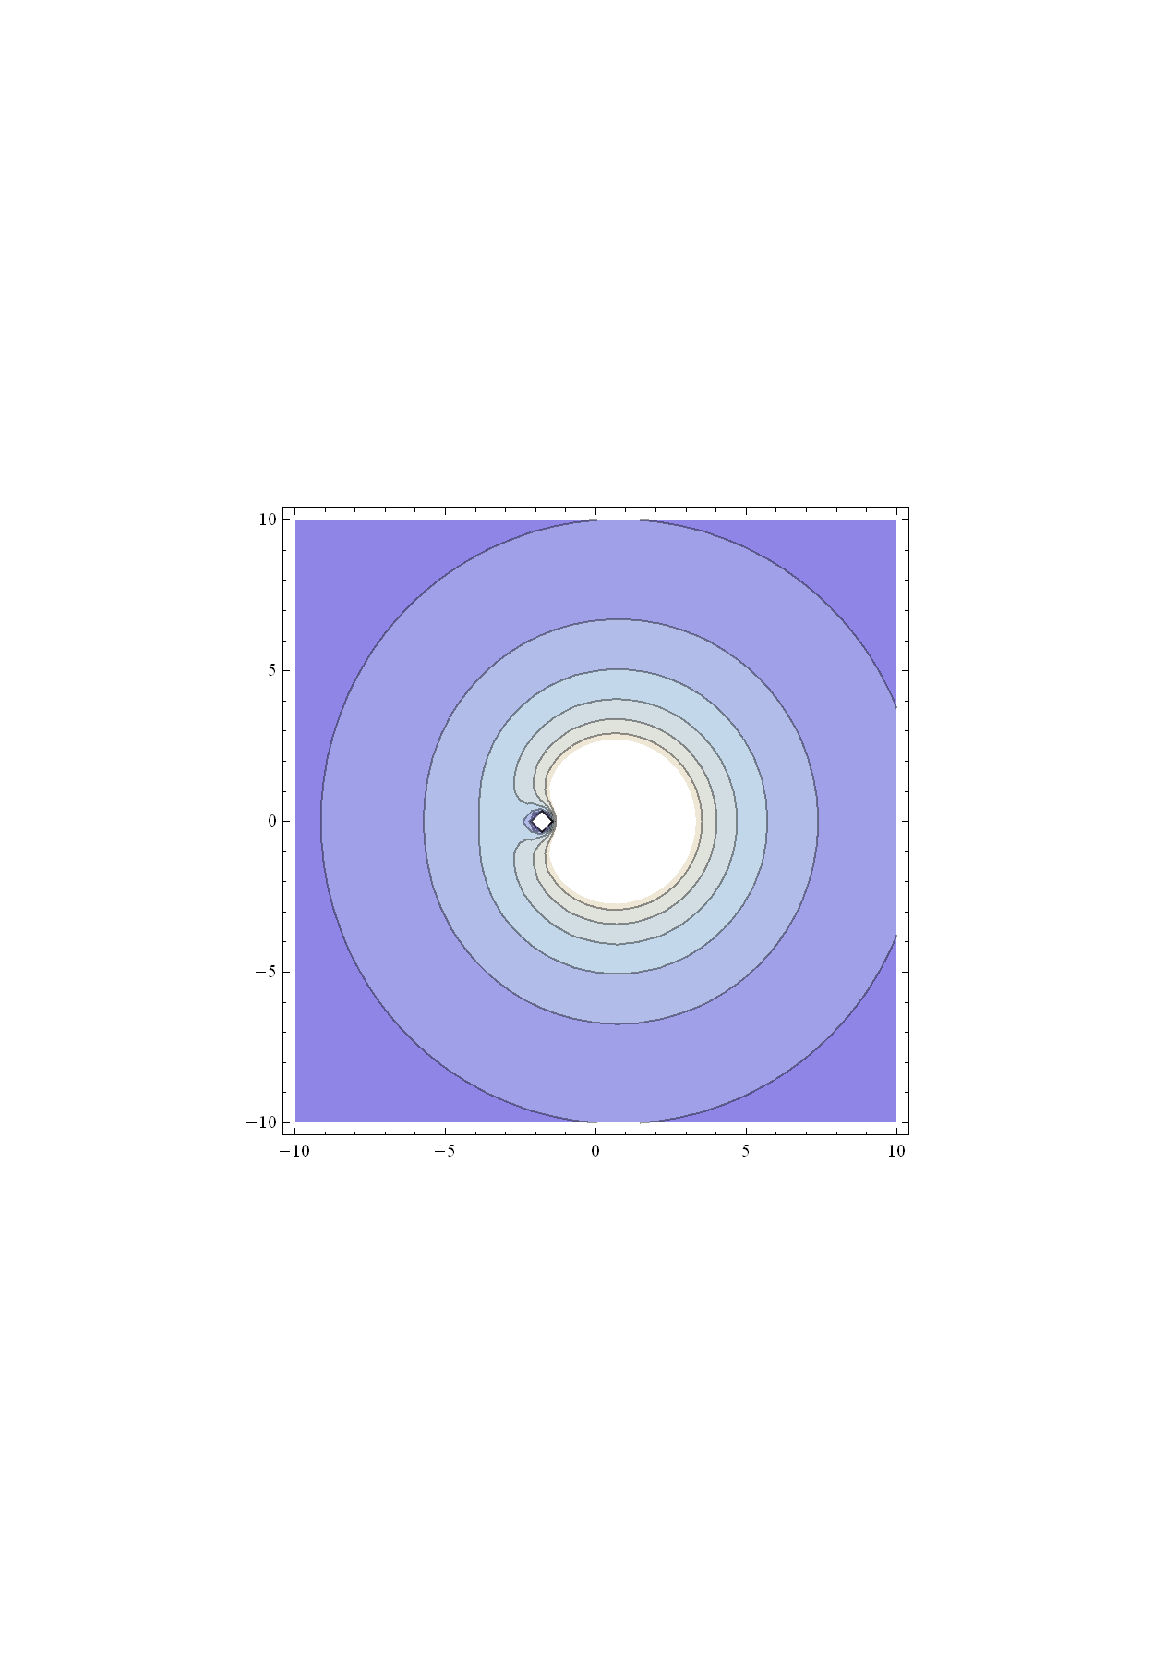
\includegraphics[width=7.265cm,height=7.165cm]{odt15-img016.emf}
 \par}
\centering а) Двухцентровый
потенциал &
{\centering   [Warning: Image ignored] % Unhandled or unsupported graphics:
%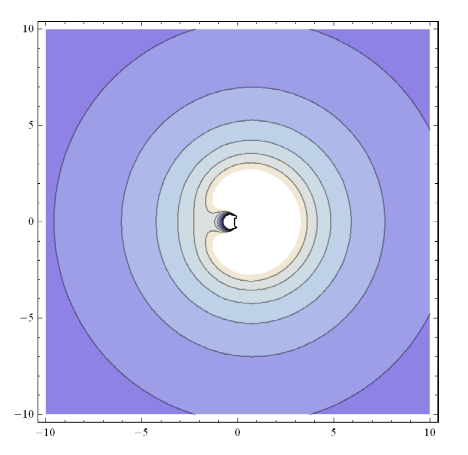
\includegraphics[width=7.303cm,height=7.2cm]{odt15-img017.emf}
 \par}
\centering\arraybslash б)
Двухцентровый
потенциал\\
\multicolumn{2}{m{16.681cm}}{\centering Рис.2}\\
\end{supertabular}
\end{flushleft}

\bigskip


\bigskip


\bigskip

\clearpage\section{Глава 2 Расчет
сил осцилляторов}
\subsection[2.1 Расчеты ab
initio]{2.1 Расчеты \foreignlanguage{english}{ab}
\foreignlanguage{english}{initio}}

В работе мы планируем исследовать молекулы $NaHe$, $CaF$, $NeH$. 
Часть параметров, которые нам необходимы для использования метода $QDT$, мы можем узнать, произведя компьютерный расчет $ab initio$ основного состояния ионов соответствующих молекул.
Такими параметрами являются вращательные константы, дипольные и квадрупольные моменты. 
Будем использовать для этого программы \foreignlanguage{english}{Gaussian 09W} и \foreignlanguage{english}{GaussView} 5.0.

Пример кода программы для расчета оптимальной конфигурации иона
\foreignlanguage{english}{NaHe}+.

\foreignlanguage{english}{\#p opt MP4/aug-cc-pV5Z}

\foreignlanguage{english}{NaHe}

\foreignlanguage{english}{1 1}

\foreignlanguage{english}{Na \ \ \ \ \ \ \ \ \ \ \ \ }

\foreignlanguage{english}{He 1 R}

\foreignlanguage{english}{R 2.31}

Видно, что производится оптимизация межъядерного расстояния в ионе \foreignlanguage{english}{NaHe}+ методом Мольера--Плиссе 4-го порядка (\foreignlanguage{english}{MP}4) с используемым базисом aug-cc-pV5Z. 
Для молекулы \foreignlanguage{english}{CaF} были использованы экспериментальные результаты,
полученные \foreignlanguage{english}{Jungen} в 2001 году.

Приведем для каждого иона сводную таблицу полученных результатов.

\begin{flushleft}
\tablefirsthead{}
\tablehead{}
\tabletail{}
\tablelasttail{}
\begin{supertabular}{|m{1.495cm}|m{2.3539999cm}|m{2.781cm}|m{2.76cm}|m{2.899cm}|m{2.9359999cm}|}
\hline
\textbf{\textcolor{black}{Метод расчета}} &
\textbf{\textcolor{black}{Базис}} &
\textbf{\textcolor{black}{B (а.е.)}} &
\textbf{\textcolor{black}{Дипольный
момент, a.u.}} &
\textbf{\textcolor{black}{Квадрупольный
момент, a.u.}} &
\textbf{\textcolor{black}{Эффективный
дипольный момент,
a.u.}}\\\hline
\centering \textcolor{black}{MP2} &
\textcolor{black}{6-31++g} &
\raggedleft  $5,14\ast 10^{-7}$ &
\raggedleft \textcolor{black}{0,65} &
\raggedleft \textcolor{black}{0,20} &
\raggedleft\arraybslash \textcolor{black}{0,47}\\\hline
\centering \textcolor{black}{MP4} &
\textcolor{black}{6-31++g} &
\raggedleft  $5,11\ast 10^{-7}$ &
\raggedleft \textcolor{black}{0,75} &
\raggedleft \textcolor{black}{0,24} &
\raggedleft\arraybslash \textcolor{black}{0,57}\\\hline
 &
\textcolor{black}{aug-cc-pVTZ} &
\raggedleft  $6,13\ast 10^{-7}$ &
\raggedleft \textit{\textcolor{black}{0,60}} &
\raggedleft \textit{\textcolor{black}{0,30}} &
\raggedleft\arraybslash \textcolor{black}{0,24}\\\hhline{~-----}
 &
\textcolor{black}{aug-cc-pV5Z} &
\raggedleft  $6,13\ast 10^{-7}$ &
\raggedleft \textit{\textcolor{black}{0,60}} &
\raggedleft \textit{\textcolor{black}{0,30}} &
\raggedleft\arraybslash \textcolor{black}{0,24}\\\hline
\centering \textcolor{black}{HF} &
\textcolor{black}{6-31++g} &
\raggedleft  $5,11\ast 10^{-7}$ &
\raggedleft \textit{\textcolor{black}{0,75}} &
\raggedleft \textit{\textcolor{black}{0,24}} &
\raggedleft\arraybslash \textcolor{black}{0,57}\\\hline
 &
\textcolor{black}{aug-cc-pVTZ} &
\raggedleft  $6,14\ast 10^{-7}$ &
\raggedleft \textcolor{black}{0,64} &
\raggedleft \textcolor{black}{0,32} &
\raggedleft\arraybslash \textcolor{black}{0,30}\\\hline
\centering \textcolor{black}{CCSD(T)} &
\textcolor{black}{6-31++g} &
\raggedleft  $5,11\ast 10^{-7}$ &
\raggedleft \textcolor{black}{0,75} &
\raggedleft \textcolor{black}{0,24} &
\raggedleft\arraybslash \textcolor{black}{0,57}\\\hline
 &
\textcolor{black}{aug-cc-pVTZ} &
\raggedleft  $6,14\ast 10^{-7}$ &
\raggedleft \textcolor{black}{0,64} &
\raggedleft \textcolor{black}{0,32} &
\raggedleft\arraybslash \textcolor{black}{0,30}\\\hhline{~-----}
\end{supertabular}
\end{flushleft}
{\centering
\textcolor{black}{Таблица 4. Ион NaHe+}
\par}


\bigskip

\begin{flushleft}
\tablefirsthead{}
\tablehead{}
\tabletail{}
\tablelasttail{}
\begin{supertabular}{|m{1.8989999cm}|m{2.476cm}|m{2.2979999cm}|m{2.294cm}|m{2.917cm}|m{3.2849998cm}|}
\hline
\textbf{\textcolor{black}{Метод расчета}} &
\textbf{{Базис}} &
\textbf{{B (а.е.)}} &
\textbf{{Дипольный
момент, a.u.}} &
\textbf{{Квадрупольный
момент, a.u.}} &
\textbf{{Эффективный
дипольный момент,
a.u.}}\\\hline
\centering {MP2} &
{6-31++g} &
\raggedleft  $2,14\ast 10^{-7}$ &
\raggedleft {5,00} &
\raggedleft {{}-1,28} &
\raggedleft\arraybslash {5,13}\\\hline
\centering {MP4} &
{6-31++g} &
\raggedleft  $2,14\ast 10^{-7}$ &
\raggedleft {5,02} &
\raggedleft {{}-1,29} &
\raggedleft\arraybslash {5,15}\\\hline
 &
{aug-cc-pVTZ} &
{{}-{}-} &
~
 &
~
 &
~
\\\hhline{~-----}
 &
{aug-cc-pV5Z} &
{{}-{}-} &
~
 &
~
 &
~
\\\hline
\centering {HF} &
{6-31++g} &
\raggedleft  $2,23\ast 10^{-7}$ &
\raggedleft \textit{{4,91}} &
\raggedleft \textit{{{}-1,26}} &
\raggedleft\arraybslash {5,04}\\\hline
 &
{aug-cc-pVTZ} &
{{}-{}-} &
~
 &
~
 &
~
\\\hline
\centering {CCSD(T)} &
{6-31++g} &
\raggedleft  $2,15\ast 10^{-7}$ &
\raggedleft {5,00} &
\raggedleft {{}-1,29} &
\raggedleft\arraybslash {5,12}\\\hline
 &
{aug-cc-pVTZ} &
{{}-{}-} &
~
 &
~
 &
~
\\\hhline{------}
\end{supertabular}
\end{flushleft}
{\centering
{Таблица 5. Ион
}\foreignlanguage{english}{{CaF}}{+}
\par}

\begin{flushleft}
\tablefirsthead{}
\tablehead{}
\tabletail{}
\tablelasttail{}
\begin{supertabular}{|m{1.813cm}|m{2.536cm}|m{2.284cm}|m{2.245cm}|m{2.8969998cm}|m{3.405cm}|}
\hline
\textbf{{Метод расчета}} &
\textbf{{Базис}} &
\textbf{{B (а.е.)}} &
\textbf{{Дипольный
момент, a.u.}} &
\textbf{{Квадрупольный
момент, a.u.}} &
\textbf{{Эффективный
дипольный момент,
a.u.}}\\\hline
\centering {MP2} &
{6-31++g} &
\raggedleft  $1,11\ast 10^{-5}$ &
\raggedleft {1,40} &
\raggedleft {0,94} &
\raggedleft\arraybslash {1,01}\\\hline
\centering {MP4} &
{6-31++g} &
\raggedleft  $1,11\ast 10^{-5}$ &
\raggedleft {1,40} &
\raggedleft {0,94} &
\raggedleft\arraybslash {1,01}\\\hline
 &
{aug-cc-pVTZ} &
\raggedleft  $1,29\ast 10^{-5}$ &
\raggedleft \textit{{1,17}} &
\raggedleft {0,89} &
\raggedleft\arraybslash {0,70}\\\hhline{------}
 &
{aug-cc-pV5Z} &
\foreignlanguage{english}{{{}-{}-{}-}} &
\foreignlanguage{english}{\textit{{{}-{}-{}-}}} &
\foreignlanguage{english}{\textit{{{}-{}-{}-}}} &
~
\\\hline
\centering {HF} &
{6-31++g} &
\raggedleft  $1,16\ast 10^{-5}$ &
\raggedleft \textit{{1,35}} &
\raggedleft \textit{{0,90}} &
\raggedleft\arraybslash {0,97}\\\hline
 &
{aug-cc-pVTZ} &
\raggedleft  $1,35\ast 10^{-5}$ &
\raggedleft {1,07} &
\raggedleft {0,77} &
\raggedleft\arraybslash {0,61}\\\hline
\centering {CCSD(T)} &
{6-31++g} &
\raggedleft  $1,11\ast 10^{-5}$ &
\raggedleft {1,39} &
\raggedleft {0,94} &
\raggedleft\arraybslash {1,00}\\\hline
 &
{aug-cc-pVTZ} &
\raggedleft  $1,29\ast 10^{-5}$ &
\raggedleft {1,10} &
\raggedleft {0,81} &
\raggedleft\arraybslash {0,64}\\\hhline{------}
\end{supertabular}
\end{flushleft}
{\centering
{Таблица
}\foreignlanguage{english}{{6}}{. Ион
}\foreignlanguage{english}{{NeH}}{+}
\par}

\subsection{2.2 Определение
применимости прямого приближения
Борна-Оппенгеймера.}
Определим, при каких условиях для исследуемых молекул выполняется
соотношение  $(1.1)$,
которое позволяет использовать прямое приближение Борна-Оппенгеймера.

\begin{equation*}
4\mathit{BJ}{\ll}\frac{\mu }{n^3}
\end{equation*}
Среди серий берем серию с минимальным квантовым дефектом. Квантовый дефект усредняем по
\foreignlanguage{english}{\textit{n}}\textit{.} Для каждой
молекулы
оцениваем \foreignlanguage{english}{\textit{n}}\textit{,
}при котором
соотношение перестает выполняться.

\begin{flushleft}
\tablefirsthead{}
\tablehead{}
\tabletail{}
\tablelasttail{}
\begin{supertabular}{|m{2.102cm}|m{1.8969998cm}|m{2.7319999cm}|m{3.726cm}|m{4.353cm}|}
\hline
\textbf{{Молекула}} &
\textbf{{{\textmu}}} &
\textbf{{Серия}} &
\textbf{{B (а.е.)}} &
\textbf{{n}}\\\hline
{NaHe} &
\raggedleft {{}-0,089} &
{Пd} &
\raggedleft  $6,175\ast 10^{-7}$ &
\raggedleft\arraybslash {33}\\\hline
{CaF} &
\raggedleft {0,023} &
{$\Delta $f} &
\raggedleft  $2,126\ast 10^{-7}$ &
\raggedleft\arraybslash {30}\\\hline
{NeH} &
\raggedleft {{}-0,03}\foreignlanguage{english}{{9}} &
{$\Sigma $d} &
\raggedleft  $1,295\ast 10^{-5}$ &
\raggedleft\arraybslash {9}\\\hline
\end{supertabular}
\end{flushleft}
{\centering
{Таблица }\foreignlanguage{english}{{4}}
\par}

Видно, что соотношение перестает выполняться при достаточно
больших \foreignlanguage{english}{\textit{n}}.

\subsection[2.3 Значения сил
осцилляторов для молекулы NaHe. Запрещенные
переходы.]{2.3
Значения сил осцилляторов для
молекулы \foreignlanguage{english}{NaHe}.
Запрещенные
переходы.}
{\centering
\textbf{Зависимость
квантового
дефекта от }\foreignlanguage{english}{\textbf{n}}\textbf{
для }\foreignlanguage{english}{\textbf{NaHe}}
\par}

Квантовые дефекты приведены по
статье T\foreignlanguage{english}{heodorakopoulus}
\foreignlanguage{english}{G}. \foreignlanguage{english}{and} \foreignlanguage{english}{Petsalakis},.
\foreignlanguage{english}{D.} 1993\foreignlanguage{english}{ }года
\foreignlanguage{english}{[19]}


\bigskip

{\centering
\textbf{Силы
осцилляторов (NaHe)}
\par}

\begin{flushleft}
\tablefirsthead{}
\tablehead{}
\tabletail{}
\tablelasttail{}
\begin{supertabular}{|m{4.3650002cm}|m{5.1150002cm}|m{5.464cm}|}
\hline
\textbf{{Переход}} &
\textbf{{f }}\textbf{{\textsubscript{osc }}}\textbf{{* 1000}} &
\textbf{{f }}\textbf{{\textsubscript{osc}}}\textbf{{ * 1000
}}\foreignlanguage{english}{\textbf{{[17]}}}\\\hline
{$\Sigma $ (3s) $\rightarrow $ П (3p)} &
\raggedleft {55}\foreignlanguage{english}{{3}} &
\raggedleft\arraybslash {561}\\
{$\Sigma $ (3s) $\rightarrow $ П (4p)} &
\raggedleft {0,5}\foreignlanguage{english}{{1}} &
\raggedleft\arraybslash {6,41}\\
{$\Sigma $ (3s) $\rightarrow $ П (5p)} &
\raggedleft {1,3}\foreignlanguage{english}{{1}} &
\raggedleft\arraybslash {1,33}\\
{$\Sigma $ (3s) $\rightarrow $ П (6p)} &
\raggedleft {0,16}\foreignlanguage{english}{{3}} &
\raggedleft\arraybslash {0,165}\\
{$\Sigma $ (3s) $\rightarrow $ П (7p)} &
\raggedleft {0,0942} &
\raggedleft\arraybslash {0,0947}\\
{$\Sigma $ (3s) $\rightarrow $ П (8p)} &
\raggedleft {0,0208} &
\raggedleft\arraybslash {0,0215}\\
{$\Sigma $ (3s) $\rightarrow $ П (9p)} &
\raggedleft {0,01}\foreignlanguage{english}{{2}} &
\raggedleft\arraybslash {0,011}\\
{$\Sigma $ (3s) $\rightarrow $ П (10p)} &
\raggedleft {0,0065}\foreignlanguage{english}{{2}} &
\raggedleft\arraybslash {0,00644}\\\hline
{$\Sigma $ (5s) $\rightarrow $ П (5p)} &
\raggedleft {1168} &
\raggedleft\arraybslash {1190}\\
{$\Sigma $ (5s) $\rightarrow $ П (6p)} &
\raggedleft {79,}\foreignlanguage{english}{{1}} &
\raggedleft\arraybslash {80,3}\\
{$\Sigma $ (5s) $\rightarrow $ П (7p)} &
\raggedleft {23,6} &
\raggedleft\arraybslash {24}\foreignlanguage{english}{{,0}}\\
{$\Sigma $ (5s) $\rightarrow $ П (8p)} &
\raggedleft {9,47} &
\raggedleft\arraybslash {9,64}\\
{$\Sigma $ (5s) $\rightarrow $ П (9p)} &
\raggedleft {5,1}\foreignlanguage{english}{{5}} &
\raggedleft\arraybslash {5,18}\\
{$\Sigma $ (5s) $\rightarrow $ П (10p)} &
\raggedleft {2,0}\foreignlanguage{english}{{6}} &
\raggedleft\arraybslash {2,09}\\\hline
{$\Sigma $ (3p) $\rightarrow $ $\Sigma $ (4s)} &
\raggedleft {15}\foreignlanguage{english}{{7}} &
\raggedleft\arraybslash {166}\\
{$\Sigma $ (3p) $\rightarrow $ $\Sigma $ (5s)} &
\raggedleft {1,1}\foreignlanguage{english}{{2}} &
\raggedleft\arraybslash {1,18}\\
{$\Sigma $ (3p) $\rightarrow $ $\Sigma $ (6s)} &
\raggedleft {0,18} &
\raggedleft\arraybslash {0,19}\\
{$\Sigma $ (3p) $\rightarrow $ $\Sigma $ (7s)} &
\raggedleft {0,094} &
\raggedleft\arraybslash {0,099}\\
{$\Sigma $ (3p) $\rightarrow $ $\Sigma $ (8s)} &
\raggedleft {0,037} &
\raggedleft\arraybslash {0,039}\\\hline
{П (3p) $\rightarrow $ $\Sigma $ (4s)} &
\raggedleft {13}\foreignlanguage{english}{{3}} &
\raggedleft\arraybslash {135}\\
{П (3p) $\rightarrow $ $\Sigma $ (5s)} &
\raggedleft {3,78} &
\raggedleft\arraybslash {3,83}\\
{П (3p) $\rightarrow $ $\Sigma $ (6s)} &
\raggedleft {0,351} &
\raggedleft\arraybslash {0,355}\\
{П (3p) $\rightarrow $ $\Sigma $ (7s)} &
\raggedleft {0,11}\foreignlanguage{english}{{6}} &
\raggedleft\arraybslash {0,117}\\
{П (3p) $\rightarrow $ $\Sigma $ (8s)} &
\raggedleft {0,028}\foreignlanguage{english}{{5}} &
\raggedleft\arraybslash {0,0285}\\\hline
{П (4p) $\rightarrow $ $\Sigma $ (5s)} &
\raggedleft {27}\foreignlanguage{english}{{9}} &
\raggedleft\arraybslash {283}\\
{П (4p) $\rightarrow $ $\Sigma $ (6s)} &
\raggedleft {18,5} &
\raggedleft\arraybslash {18,8}\\
{П (4p) $\rightarrow $ $\Sigma $ (7s)} &
\raggedleft {5,95} &
\raggedleft\arraybslash {6,04}\\
{П (4p) $\rightarrow $ $\Sigma $ (8s)} &
\raggedleft {2,6}\foreignlanguage{english}{{6}} &
\raggedleft\arraybslash {2,7}\\
{П (4p) $\rightarrow $ $\Sigma $ (9s)} &
\raggedleft {1,8}\foreignlanguage{english}{{5}} &
\raggedleft\arraybslash {1,87}\\
{П (4p) $\rightarrow $ $\Sigma $ (10s)} &
\raggedleft {1,11} &
\raggedleft\arraybslash {1,13}\\\hline
{П (5p) $\rightarrow $ $\Sigma $ (6s)} &
\raggedleft {427} &
\raggedleft\arraybslash {434}\\
{П (5p) $\rightarrow $ $\Sigma $ (7s)} &
\raggedleft {15,3} &
\raggedleft\arraybslash {15,5}\\
{П (5p) $\rightarrow $ $\Sigma $ (8s)} &
\raggedleft {4,0} &
\raggedleft\arraybslash {4,1}\\
{П (5p) $\rightarrow $ $\Sigma $ (9s)} &
\raggedleft {2,}\foreignlanguage{english}{{90}} &
\raggedleft\arraybslash {2,94}\\
{П (5p) $\rightarrow $ $\Sigma $ (10s)} &
\raggedleft {1,49} &
\raggedleft\arraybslash {1,51}\\\hline
{П (6p) $\rightarrow $ $\Sigma $ (7s)} &
\raggedleft {56}\foreignlanguage{english}{{9}} &
\raggedleft\arraybslash {577}\\
{П (6p) $\rightarrow $ $\Sigma $ (8s)} &
\raggedleft {20,4} &
\raggedleft\arraybslash {20,7}\\
{П (6p) $\rightarrow $ $\Sigma $ (9s)} &
\raggedleft {8,83} &
\raggedleft\arraybslash {8,95}\\
{П (6p) $\rightarrow $ $\Sigma $ 10s)} &
\raggedleft {3,7}\foreignlanguage{english}{{6}} &
\raggedleft\arraybslash {3,8}\\\hline
{П (7p) $\rightarrow $ $\Sigma $ (8s)} &
\raggedleft {70}\foreignlanguage{english}{{3}} &
\raggedleft\arraybslash {713}\\
{П (7p) $\rightarrow $ $\Sigma $ (9s)} &
\raggedleft {33,}\foreignlanguage{english}{{1}} &
\raggedleft\arraybslash {33,6}\\
{П (7p) $\rightarrow $ $\Sigma $ (10s)} &
\raggedleft {8,83} &
\raggedleft\arraybslash {8,95}\\\hline
{П (8p) $\rightarrow $ $\Sigma $ (9s)} &
\raggedleft {839} &
\raggedleft\arraybslash {852}\\
{П (8p) $\rightarrow $ $\Sigma $ (10s)} &
\raggedleft {38,0} &
\raggedleft\arraybslash {38,4}\\\hline
{П (9p) $\rightarrow $ $\Sigma $ (10s)} &
\raggedleft {980} &
\raggedleft\arraybslash {995}\\\hline
{$\Sigma $ (3p) $\rightarrow $ П (3d)} &
\raggedleft {4}\foreignlanguage{english}{{70}} &
\raggedleft\arraybslash {470}\\
{$\Sigma $ (3p) $\rightarrow $ П (4d)} &
\raggedleft
{4}\foreignlanguage{english}{{1}}{,}\foreignlanguage{english}{{0}}
&
\raggedleft\arraybslash {41,1}\\
{$\Sigma $ (3p) $\rightarrow $ П (5d)} &
\raggedleft {12,}\foreignlanguage{english}{{4}} &
\raggedleft\arraybslash {12,4}\\
{$\Sigma $ (3p) $\rightarrow $ П (6d)} &
\raggedleft {6,24} &
\raggedleft\arraybslash {6,26}\\
{$\Sigma $ (3p) $\rightarrow $ П (7d)} &
\raggedleft {2,}\foreignlanguage{english}{{30}} &
\raggedleft\arraybslash {2,31}\\
{$\Sigma $ (3p) $\rightarrow $ П (8d)} &
\raggedleft {0,81}\foreignlanguage{english}{{4}} &
\raggedleft\arraybslash {0,814}\\
{$\Sigma $ (3p) $\rightarrow $ П (9d)} &
\raggedleft {1,64} &
\raggedleft\arraybslash {1,65}\\
{$\Sigma $ (3p) $\rightarrow $ П (10d)} &
\raggedleft {1,0}\foreignlanguage{english}{{7}} &
\raggedleft\arraybslash {1,07}\\\hline
{П(3p) $\rightarrow $ $\Sigma $ (3d)} &
\raggedleft {75,7} &
\raggedleft\arraybslash {76,4}\\
{П(3p) $\rightarrow $ $\Sigma $ (4d)} &
\raggedleft {7,9}\foreignlanguage{english}{{1}} &
\raggedleft\arraybslash {7,97}\\
{П(3p) $\rightarrow $ $\Sigma $ (5d)} &
\raggedleft {3,1}\foreignlanguage{english}{{5}} &
\raggedleft\arraybslash {3,18}\\
{П(3p) $\rightarrow $ $\Sigma $ (6d)} &
\raggedleft {1,60} &
\raggedleft\arraybslash {1,62}\\
{П(3p) $\rightarrow $ $\Sigma $ (7d)} &
\raggedleft {0,947} &
\raggedleft\arraybslash {0,955}\\
{П(3p) $\rightarrow $ $\Sigma $ (8d)} &
\raggedleft {0,576} &
\raggedleft\arraybslash {0,581}\\
{П(3p) $\rightarrow $ $\Sigma $ (9d)} &
\raggedleft {0,414} &
\raggedleft\arraybslash {0,418}\\
{П(3p) $\rightarrow $ $\Sigma $ (10d)} &
\raggedleft {0,29}\foreignlanguage{english}{{9}} &
\raggedleft\arraybslash {0,301}\\\hline
{П(4p) $\rightarrow $ $\Sigma $ (4d)} &
\raggedleft {70,4} &
\raggedleft\arraybslash {71}\foreignlanguage{english}{{,0}}\\
{П(4p) $\rightarrow $ $\Sigma $ (5d)} &
\raggedleft {9,24} &
\raggedleft\arraybslash {9,32}\\
{П(4p) $\rightarrow $ $\Sigma $ (6d)} &
\raggedleft {3,7}\foreignlanguage{english}{{2}} &
\raggedleft\arraybslash {3,75}\\
{П(4p) $\rightarrow $ $\Sigma $ (7d)} &
\raggedleft {2,}\foreignlanguage{english}{{10}} &
\raggedleft\arraybslash {2,12}\\
{П(4p) $\rightarrow $ $\Sigma $ (8d)} &
\raggedleft {1,25} &
\raggedleft\arraybslash {1,26}\\
{П(4p) $\rightarrow $ $\Sigma $ (9d)} &
\raggedleft {0,759} &
\raggedleft\arraybslash {0,765}\\
{П(4p) $\rightarrow $ $\Sigma $ (10d)} &
\raggedleft {0,539} &
\raggedleft\arraybslash {0,543}\\\hline
{П(5p) $\rightarrow $ $\Sigma $ (5d)} &
\raggedleft {92,9} &
\raggedleft\arraybslash {93,7}\\
{П(5p) $\rightarrow $ $\Sigma $ (6d)} &
\raggedleft {12,9} &
\raggedleft\arraybslash {13}\\
{П(5p) $\rightarrow $ $\Sigma $ (7d)} &
\raggedleft {5,2}\foreignlanguage{english}{{9}} &
\raggedleft\arraybslash {5,33}\\
{П(5p) $\rightarrow $ $\Sigma $ (8d)} &
\raggedleft {2,54} &
\raggedleft\arraybslash {2,57}\\
{П(5p) $\rightarrow $ $\Sigma $ (9d)} &
\raggedleft {1,6}\foreignlanguage{english}{{1}} &
\raggedleft\arraybslash {1,62}\\
{П(5p) $\rightarrow $ $\Sigma $ (10d)} &
\raggedleft {1,0}\foreignlanguage{english}{{7}} &
\raggedleft\arraybslash {1,08}\\
\end{supertabular}
\end{flushleft}
\foreignlanguage{english}{$\rightarrow $}

{\centering
\textbf{Запрещенные
переходы}
\par}

\begin{flushleft}
\tablefirsthead{}
\tablehead{}
\tabletail{}
\tablelasttail{}
\begin{supertabular}{|m{5.076cm}|m{5.302cm}|}
\hline
\textbf{{Переход}} &
\textbf{{f }}\textbf{{\textsubscript{osc}}}\textbf{{ * 1000}}\\\hline
{$\Sigma $ (3s) $\rightarrow $ $\Sigma $ (3d)} &
\raggedleft\arraybslash {0,9753}\\
{$\Sigma $ (3s) $\rightarrow $ $\Sigma $ (4d)} &
\raggedleft\arraybslash {0,2788}\\
{$\Sigma $ (3s) $\rightarrow $ $\Sigma $ (5d)} &
\raggedleft\arraybslash {0,1250}\\
{$\Sigma $ (3s) $\rightarrow $ $\Sigma $ (6d)} &
\raggedleft\arraybslash {0,0684}\\
{$\Sigma $ (3s) $\rightarrow $ $\Sigma $ (7d)} &
\raggedleft\arraybslash {0,0398}\\
{$\Sigma $ (3s) $\rightarrow $ $\Sigma $ (8d)} &
\raggedleft\arraybslash {0,0242}\\\hline
{$\Sigma $ (3s) $\rightarrow $ П (3d)} &
\raggedleft\arraybslash {1,5158}\\
{$\Sigma $ (3s) $\rightarrow $ П (4d)} &
\raggedleft\arraybslash {0,4192}\\
{$\Sigma $ (3s) $\rightarrow $ П (5d)} &
\raggedleft\arraybslash {0,1879}\\
{$\Sigma $ (3s) $\rightarrow $ П (6d)} &
\raggedleft\arraybslash {0,1029}\\
{$\Sigma $ (3s) $\rightarrow $ П (7d)} &
\raggedleft\arraybslash {0,0598}\\
{$\Sigma $ (3s) $\rightarrow $ П (8d)} &
\raggedleft\arraybslash {0,0364}\\\hline
{$\Sigma $ (3d) $\rightarrow $ $\Sigma $ (5p)} &
\raggedleft\arraybslash {0,2894}\\
{$\Sigma $ (3d) $\rightarrow $ $\Sigma $ (6p)} &
\raggedleft\arraybslash {0,0297}\\
{$\Sigma $ (3d) $\rightarrow $ $\Sigma $ (7p)} &
\raggedleft\arraybslash {0,0095}\\
{$\Sigma $ (3d) $\rightarrow $ $\Sigma $ (8p)} &
\raggedleft\arraybslash {0,0045}\\\hline
{П (3d) $\rightarrow $ П (5p)} &
\raggedleft\arraybslash {0,2008}\\
{П (3d) $\rightarrow $ П (6p)} &
\raggedleft\arraybslash {0,0222}\\
{П (3d) $\rightarrow $ П (7p)} &
\raggedleft\arraybslash {0,0072}\\
{П (3d) $\rightarrow $ П (8p)} &
\raggedleft\arraybslash {0,0034}\\\hline
\end{supertabular}
\end{flushleft}

\bigskip

\subsection[2.4 Значения сил
осцилляторов для молекулы CaF. Запрещенные
переходы.]{2.4
Значения сил осцилляторов для
молекулы \foreignlanguage{english}{CaF}.
Запрещенные
переходы.}
{\centering
\textbf{Зависимость
квантового
дефекта от }\foreignlanguage{english}{\textbf{n}}\textbf{
для }\foreignlanguage{english}{\textbf{CaF}}
\par}

Квантовые дефекты приведены по
статье Jungen \& A. L. Roche 1997 [18].


\bigskip

{\centering
\textbf{Силы
осцилляторов
(}\foreignlanguage{english}{\textbf{CaF}}\textbf{)}
\par}

\begin{flushleft}
\tablefirsthead{}
\tablehead{}
\tabletail{}
\tablelasttail{}
\begin{supertabular}{|m{6.577cm}|m{6.801cm}|}
\hline
\textbf{{Переход}} &
\textbf{{f }}\textbf{{\textsubscript{osc }}}\textbf{{* 1000}}\\\hline
{$\Sigma $ (3s) $\rightarrow $ П (3p)} &
\raggedleft\arraybslash {540,646}\\
{$\Sigma $ (3s) $\rightarrow $ П (4p)} &
\raggedleft\arraybslash {2,63634}\\
{$\Sigma $ (3s) $\rightarrow $ П (5p)} &
\raggedleft\arraybslash {0,0852597}\\\hline
{$\Sigma $ (5s) $\rightarrow $ П (5p)} &
\raggedleft\arraybslash {895,043}\\
{$\Sigma $ (5s) $\rightarrow $ П (6p)} &
\raggedleft\arraybslash {11,6609}\\
{$\Sigma $ (5s) $\rightarrow $ П (7p)} &
\raggedleft\arraybslash {1,58738}\\
{$\Sigma $ (5s) $\rightarrow $ П (8p)} &
\raggedleft\arraybslash {0,418616}\\\hline
{$\Sigma $ (3p) $\rightarrow $ $\Sigma $ (4s)} &
\raggedleft\arraybslash {41,8333}\\
{$\Sigma $ (3p) $\rightarrow $ $\Sigma $ (5s)} &
\raggedleft\arraybslash {4,96279}\\
{$\Sigma $ (3p) $\rightarrow $ $\Sigma $ (6s)} &
\raggedleft\arraybslash {1,70301}\\
{$\Sigma $ (3p) $\rightarrow $ $\Sigma $ (7s)} &
\raggedleft\arraybslash {0,819515}\\
{$\Sigma $ (3p) $\rightarrow $ $\Sigma $ (8s)} &
\raggedleft\arraybslash {0,467}\\\hline
{П (3p) $\rightarrow $ $\Sigma $ (4s)} &
\raggedleft\arraybslash {152,939}\\
{П (3p) $\rightarrow $ $\Sigma $ (5s)} &
\raggedleft\arraybslash {14,91}\\
{П (3p) $\rightarrow $ $\Sigma $ (6s)} &
\raggedleft\arraybslash {4,91959}\\
{П (3p) $\rightarrow $ $\Sigma $ (7s)} &
\raggedleft\arraybslash {2,33021}\\
{П (3p) $\rightarrow $ $\Sigma $ (8s)} &
\raggedleft\arraybslash {1,31702}\\\hline
{П (4p) $\rightarrow $ $\Sigma $ (5s)} &
\raggedleft\arraybslash {229,818}\\
{П (4p) $\rightarrow $ $\Sigma $ (6s)} &
\raggedleft\arraybslash {21,7936}\\
{П (4p) $\rightarrow $ $\Sigma $ (7s)} &
\raggedleft\arraybslash {7,18156}\\
{П (4p) $\rightarrow $ $\Sigma $ (8s)} &
\raggedleft\arraybslash {3,42319}\\
{П (4p) $\rightarrow $ $\Sigma $ (9s)} &
\raggedleft\arraybslash {1,95175}\\
{П (4p) $\rightarrow $ $\Sigma $ (10s)} &
\raggedleft\arraybslash {1,23757}\\\hline
{П (5p) $\rightarrow $ $\Sigma $ (6s)} &
\raggedleft\arraybslash {306,423}\\
{П (5p) $\rightarrow $ $\Sigma $ (7s)} &
\raggedleft\arraybslash {28,415}\\
{П (5p) $\rightarrow $ $\Sigma $ (8s)} &
\raggedleft\arraybslash {9,3244}\\
{П (5p) $\rightarrow $ $\Sigma $ (9s)} &
\raggedleft\arraybslash {4,45211}\\
{П (5p) $\rightarrow $ $\Sigma $ (10s)} &
\raggedleft\arraybslash {2,54893}\\\hline
{П (6p) $\rightarrow $ $\Sigma $ (7s)} &
\raggedleft\arraybslash {382,835}\\
{П (6p) $\rightarrow $ $\Sigma $ (8s)} &
\raggedleft\arraybslash {34,873}\\
{П (6p) $\rightarrow $ $\Sigma $ (9s)} &
\raggedleft\arraybslash {11,3872}\\
{П (6p) $\rightarrow $ $\Sigma $ 10s)} &
\raggedleft\arraybslash {5,43507}\\\hline
{$\Sigma $ (3p) $\rightarrow $ $\Sigma $ (3d)} &
\raggedleft\arraybslash {168,154}\\
{$\Sigma $ (3p) $\rightarrow $ $\Sigma $ (4d)} &
\raggedleft\arraybslash {62,9363}\\
{$\Sigma $ (3p) $\rightarrow $ $\Sigma $ (5d)} &
\raggedleft\arraybslash {26,0193}\\
{$\Sigma $ (3p) $\rightarrow $ $\Sigma $ (6d)} &
\raggedleft\arraybslash {13,1257}\\
{$\Sigma $ (3p) $\rightarrow $ $\Sigma $ (7d)} &
\raggedleft\arraybslash {7,60738}\\
{$\Sigma $ (3p) $\rightarrow $ $\Sigma $ (8d)} &
\raggedleft\arraybslash {4,83377}\\
{$\Sigma $ (3p) $\rightarrow $ $\Sigma $ (9d)} &
\raggedleft\arraybslash {3,27671}\\
{$\Sigma $ (3p) $\rightarrow $ $\Sigma $ (10d)} &
\raggedleft\arraybslash {2,33037}\\\hline
{$\Sigma $ (3p) $\rightarrow $ П (4d)} &
\raggedleft\arraybslash {595,958}\\
{$\Sigma $ (3p) $\rightarrow $ П (5d)} &
\raggedleft\arraybslash {14,7546}\\
{$\Sigma $ (3p) $\rightarrow $ П (6d)} &
\raggedleft\arraybslash {2,8325}\\
{$\Sigma $ (3p) $\rightarrow $ П (7d)} &
\raggedleft\arraybslash {0,993477}\\
{$\Sigma $ (3p) $\rightarrow $ П (8d)} &
\raggedleft\arraybslash {0,46517}\\
{$\Sigma $ (3p) $\rightarrow $ П (9d)} &
\raggedleft\arraybslash {0,25745}\\
{$\Sigma $ (3p) $\rightarrow $ П (10d)} &
\raggedleft\arraybslash {0,158713}\\\hline
{П(3p) $\rightarrow $ $\Sigma $ (3d)} &
\raggedleft\arraybslash {11,3833}\\
{П(3p) $\rightarrow $ $\Sigma $ (4d)} &
\raggedleft\arraybslash {8,25686}\\
{П(3p) $\rightarrow $ $\Sigma $ (5d)} &
\raggedleft\arraybslash {2,9363}\\
{П(3p) $\rightarrow $ $\Sigma $ (6d)} &
\raggedleft\arraybslash {1,40099}\\
{П(3p) $\rightarrow $ $\Sigma $ (7d)} &
\raggedleft\arraybslash {0,789283}\\
{П(3p) $\rightarrow $ $\Sigma $ (8d)} &
\raggedleft\arraybslash {0,49317}\\
{П(3p) $\rightarrow $ $\Sigma $ (9d)} &
\raggedleft\arraybslash {0,330694}\\
{П(3p) $\rightarrow $ $\Sigma $ (10d)} &
\raggedleft\arraybslash {0,233431}\\\hline
{П(4p) $\rightarrow $ $\Sigma $ (4d)} &
\raggedleft\arraybslash {19,3527}\\
{П(4p) $\rightarrow $ $\Sigma $ (5d)} &
\raggedleft\arraybslash {5,63813}\\
{П(4p) $\rightarrow $ $\Sigma $ (6d)} &
\raggedleft\arraybslash {2,28707}\\
{П(4p) $\rightarrow $ $\Sigma $ (7d)} &
\raggedleft\arraybslash {1,16824}\\
{П(4p) $\rightarrow $ $\Sigma $ (8d)} &
\raggedleft\arraybslash {0,688109}\\
{П(4p) $\rightarrow $ $\Sigma $ (9d)} &
\raggedleft\arraybslash {0,444106}\\
{П(4p) $\rightarrow $ $\Sigma $ (10d)} &
\raggedleft\arraybslash {0,305368}\\\hline
{П(5p) $\rightarrow $ $\Sigma $ (5d)} &
\raggedleft\arraybslash {26,1325}\\
{П(5p) $\rightarrow $ $\Sigma $ (6d)} &
\raggedleft\arraybslash {4,41627}\\
{П(5p) $\rightarrow $ $\Sigma $ (7d)} &
\raggedleft\arraybslash {1,91693}\\
{П(5p) $\rightarrow $ $\Sigma $ (8d)} &
\raggedleft\arraybslash {1,01738}\\
{П(5p) $\rightarrow $ $\Sigma $ (9d)} &
\raggedleft\arraybslash {0,615726}\\
{П(5p) $\rightarrow $ $\Sigma $ (10d)} &
\raggedleft\arraybslash {0,405816}\\\hline
\end{supertabular}
\end{flushleft}
\foreignlanguage{english}{$\rightarrow $}

{\centering
\textbf{Запрещенные
переходы}
\par}

\begin{flushleft}
\tablefirsthead{}
\tablehead{}
\tabletail{}
\tablelasttail{}
\begin{supertabular}{|m{6.577cm}|m{6.801cm}|}
\hline
\textbf{{Переход}} &
\textbf{{f }}\textbf{{\textsubscript{osc}}}\textbf{{ * 1000}}\\\hline
{$\Sigma $ (3s) $\rightarrow $ $\Sigma $ (3d)} &
\raggedleft\arraybslash {5,53923}\\
{$\Sigma $ (3s) $\rightarrow $ $\Sigma $ (4d)} &
\raggedleft\arraybslash {0,00732526}\\
{$\Sigma $ (3s) $\rightarrow $ $\Sigma $ (5d)} &
\raggedleft\arraybslash {0,0422292}\\
{$\Sigma $ (3s) $\rightarrow $ $\Sigma $ (6d)} &
\raggedleft\arraybslash {0,0365621}\\
{$\Sigma $ (3s) $\rightarrow $ $\Sigma $ (7d)} &
\raggedleft\arraybslash {0,0269932}\\
{$\Sigma $ (3s) $\rightarrow $ $\Sigma $ (8d)} &
\raggedleft\arraybslash {0,0196354}\\\hline
{$\Sigma $ (3s) $\rightarrow $ П (4d)} &
\raggedleft\arraybslash {12,6473}\\
{$\Sigma $ (3s) $\rightarrow $ П (5d)} &
\raggedleft\arraybslash {1,82629}\\
{$\Sigma $ (3s) $\rightarrow $ П (6d)} &
\raggedleft\arraybslash {0,62719}\\
{$\Sigma $ (3s) $\rightarrow $ П (7d)} &
\raggedleft\arraybslash {0,297813}\\
{$\Sigma $ (3s) $\rightarrow $ П (8d)} &
\raggedleft\arraybslash {0,167596}\\\hline
{$\Sigma $ (3d) $\rightarrow $ $\Sigma $ (5p)} &
\raggedleft\arraybslash {0,0455569}\\
{$\Sigma $ (3d) $\rightarrow $ $\Sigma $ (6p)} &
\raggedleft\arraybslash {0,0138499}\\
{$\Sigma $ (3d) $\rightarrow $ $\Sigma $ (7p)} &
\raggedleft\arraybslash {0,00634081}\\
{$\Sigma $ (3d) $\rightarrow $ $\Sigma $ (8p)} &
\raggedleft\arraybslash {0,0035161}\\\hline
\end{supertabular}
\end{flushleft}
\subsection[2.4 Значения сил
осцилляторов для молекулы NeH. Запрещенные
переходы.]{2.4
Значения сил осцилляторов для
молекулы \foreignlanguage{english}{NeH}.
Запрещенные
переходы.}
{\centering
\textbf{Зависимость
квантового
дефекта от }\foreignlanguage{english}{\textbf{$\nu $}}\textbf{
для }\foreignlanguage{english}{\textbf{NeH}}\textbf{ }
\par}

Квантовые дефекты приведены по
статье \foreignlanguage{english}{S}. \foreignlanguage{english}{Raynor}
\foreignlanguage{english}{and} \foreignlanguage{english}{D}. \foreignlanguage{english}{R}.
\foreignlanguage{english}{Herschbach} (1982).


\bigskip

{\centering
\textbf{Силы
осцилляторов
(}\foreignlanguage{english}{\textbf{NeH}}\textbf{)}
\par}

\begin{flushleft}
\tablefirsthead{}
\tablehead{}
\tabletail{}
\tablelasttail{}
\begin{supertabular}{|m{5.4360003cm}|m{6.3630004cm}|m{4.584cm}|}
\hline
\textbf{{Переход}} &
\textbf{{f }}\textbf{{\textsubscript{osc }}}\textbf{{* 1000}} &
\textbf{{f }}\textbf{{\textsubscript{osc}}}\textbf{{ * 1000
[}}\foreignlanguage{english}{\textbf{{12}}}\textbf{{]}}\\\hline
{$\Sigma $ (3s) $\rightarrow $ П (3p)} &
\raggedleft {166,38} &
\raggedleft\arraybslash {150}\\
{$\Sigma $ (3s) $\rightarrow $ П (4p)} &
\raggedleft {18,08} &
\raggedleft\arraybslash {16,3}\\
{$\Sigma $ (3s) $\rightarrow $ П (5p)} &
\raggedleft {5,81} &
\raggedleft\arraybslash {5,24}\\\hline
{$\Sigma $ (3s) $\rightarrow $ $\Sigma $ (5p)} &
\raggedleft {7,61} &
\raggedleft\arraybslash {5,24}\\
{$\Sigma $ (3s) $\rightarrow $ $\Sigma $ (6p)} &
\raggedleft {3,47} &
\raggedleft\arraybslash {2,39}\\
{$\Sigma $ (3s) $\rightarrow $ $\Sigma $ (7p)} &
\raggedleft {1,90} &
\raggedleft\arraybslash {1,31}\\
{$\Sigma $ (3s) $\rightarrow $ $\Sigma $ (8p)} &
\raggedleft {1,16} &
\raggedleft\arraybslash {0,796}\\\hline
{$\Sigma $ (3p) $\rightarrow $ $\Sigma $ (4s)} &
\raggedleft {105,83} &
\raggedleft\arraybslash {72,9}\\
{$\Sigma $ (3p) $\rightarrow $ $\Sigma $ (5s)} &
\raggedleft {1,54} &
\raggedleft\arraybslash {1,06}\\
{$\Sigma $ (3p) $\rightarrow $ $\Sigma $ (6s)} &
\raggedleft {0,36} &
\raggedleft\arraybslash {0,248}\\
{$\Sigma $ (3p) $\rightarrow $ $\Sigma $ (7s)} &
\raggedleft {0,14} &
\raggedleft\arraybslash {0,097}\\
{$\Sigma $ (3p) $\rightarrow $ $\Sigma $ (8s)} &
\raggedleft {0,07} &
\raggedleft\arraybslash {0,047}\\\hline
{П (3p) $\rightarrow $ $\Sigma $ (4s)} &
\raggedleft {154,18} &
\raggedleft\arraybslash {139}\\
{П (3p) $\rightarrow $ $\Sigma $ (5s)} &
\raggedleft {0,73} &
\raggedleft\arraybslash {0,66}\\
{П (3p) $\rightarrow $ $\Sigma $ (6s)} &
\raggedleft {0,12} &
\raggedleft\arraybslash {0,112}\\
{П (3p) $\rightarrow $ $\Sigma $ (7s)} &
\raggedleft {0,04} &
\raggedleft\arraybslash {0,036}\\
{П (3p) $\rightarrow $ $\Sigma $ (8s)} &
\raggedleft {0,02} &
\raggedleft\arraybslash {0,015}\\\hline
{$\Sigma $ (3p) $\rightarrow $ $\Sigma $ (3d)} &
\raggedleft {322,68} &
\raggedleft\arraybslash {323}\\
{$\Sigma $ (3p) $\rightarrow $ $\Sigma $ (4d)} &
\raggedleft {41,36} &
\raggedleft\arraybslash {41,4}\\
{$\Sigma $ (3p) $\rightarrow $ $\Sigma $ (5d)} &
\raggedleft {13,79} &
\raggedleft\arraybslash {13,8}\\
{$\Sigma $ (3p) $\rightarrow $ $\Sigma $ (6d)} &
\raggedleft {6,44} &
\raggedleft\arraybslash {6,45}\\
{$\Sigma $ (3p) $\rightarrow $ $\Sigma $ (7d)} &
\raggedleft {3,59} &
\raggedleft\arraybslash {3,59}\\
{$\Sigma $ (3p) $\rightarrow $ $\Sigma $ (8d)} &
\raggedleft {2,22} &
\raggedleft\arraybslash {2,22}\\\hline
{$\Sigma $ (3p) $\rightarrow $ П (4d)} &
\raggedleft {63,24} &
\raggedleft\arraybslash {64,5}\\
{$\Sigma $ (3p) $\rightarrow $ П (5d)} &
\raggedleft {21,57} &
\raggedleft\arraybslash {22}\\
{$\Sigma $ (3p) $\rightarrow $ П (6d)} &
\raggedleft {10,20} &
\raggedleft\arraybslash {10,4}\\
{$\Sigma $ (3p) $\rightarrow $ П (7d)} &
\raggedleft {5,71} &
\raggedleft\arraybslash {5,82}\\
{$\Sigma $ (3p) $\rightarrow $ П (8d)} &
\raggedleft {3,56} &
\raggedleft\arraybslash {3,63}\\\hline
{П(3p) $\rightarrow $ $\Sigma $ (3d)} &
\raggedleft {88,68} &
\raggedleft\arraybslash {77,7}\\
{П(3p) $\rightarrow $ $\Sigma $ (4d)} &
\raggedleft {9,31} &
\raggedleft\arraybslash {8,16}\\
{П(3p) $\rightarrow $ $\Sigma $ (5d)} &
\raggedleft {2,81} &
\raggedleft\arraybslash {2,46}\\
{П(3p) $\rightarrow $ $\Sigma $ (6d)} &
\raggedleft {1,23} &
\raggedleft\arraybslash {1,08}\\
{П(3p) $\rightarrow $ $\Sigma $ (7d)} &
\raggedleft {0,67} &
\raggedleft\arraybslash {0,583}\\
{П(3p) $\rightarrow $ $\Sigma $ (8d)} &
\raggedleft {0,40} &
\raggedleft\arraybslash {0,353}\\\hline
\end{supertabular}
\end{flushleft}

\bigskip

{\centering
\textbf{Запрещенные
переходы}
\par}

\begin{flushleft}
\tablefirsthead{}
\tablehead{}
\tabletail{}
\tablelasttail{}
\begin{supertabular}{|m{4.9560003cm}|m{5.806cm}|m{4.176cm}|}
\hline
\textbf{{Переход}} &
\textbf{{f }}\textbf{{\textsubscript{osc}}}\textbf{{ * 1000}} &
\textbf{{f }}\textbf{{\textsubscript{osc}}}\textbf{{ * 1000
[]}}\\\hline
{$\Sigma $ (3s) $\rightarrow $ $\Sigma $ (3d)} &
\raggedleft {2,578} &
\raggedleft\arraybslash {3,89}\\
{$\Sigma $ (3s) $\rightarrow $ $\Sigma $ (4d)} &
\raggedleft {0,769} &
\raggedleft\arraybslash {1,16}\\
{$\Sigma $ (3s) $\rightarrow $ $\Sigma $ (5d)} &
\raggedleft {0,382} &
\raggedleft\arraybslash {0,576}\\
{$\Sigma $ (3s) $\rightarrow $ $\Sigma $ (6d)} &
\raggedleft {0,216} &
\raggedleft\arraybslash {0,326}\\
{$\Sigma $ (3s) $\rightarrow $ $\Sigma $ (7d)} &
\raggedleft {0,135} &
\raggedleft\arraybslash {0,203}\\
{$\Sigma $ (3s) $\rightarrow $ $\Sigma $ (8d)} &
\raggedleft {0,089} &
\raggedleft\arraybslash {0,135}\\\hline
{$\Sigma $ (3s) $\rightarrow $ П (3d)} &
\raggedleft {3,602} &
\raggedleft\arraybslash {5,13}\\
{$\Sigma $ (3s) $\rightarrow $ П (4d)} &
\raggedleft {1,095} &
\raggedleft\arraybslash {1,56}\\
{$\Sigma $ (3s) $\rightarrow $ П (5d)} &
\raggedleft {0,554} &
\raggedleft\arraybslash {0,789}\\
{$\Sigma $ (3s) $\rightarrow $ П (6d)} &
\raggedleft {0,317} &
\raggedleft\arraybslash {0,451}\\
{$\Sigma $ (3s) $\rightarrow $ П (7d)} &
\raggedleft {0,198} &
\raggedleft\arraybslash {0,282}\\
{$\Sigma $ (3s) $\rightarrow $ П (8d)} &
\raggedleft {0,132} &
\raggedleft\arraybslash {0,188}\\\hline
\end{supertabular}
\end{flushleft}






\section{Заключение}
В настоящей работе рассмотрена задача о заряженной частице в кулон-дипольном поле в прямом приближении Борна-Оппенгеймера. Рассмотрен процесс вычисления сил осцилляторов для такой частицы и, в частности, вопрос о вычислении радиальных матричных элементов в подобной системе с использованием модельного потенциала Саймонса и метода Бейтса-Дамгард, а также о вычислении угловых матричных элементов. Рассмотрен вопрос о выборе начала отсчета для вычисления дипольного момента у заряженной системы.
Произведены расчеты ab initio несколькими различными методами мультипольных моментов системы и вращательных констант, на основе этих результатов произведен анализ применимости прямого приближения Борна-Оппенгеймера для рассматриваемых молекул NaHe, NeH и CaF. Произведено на основе метода QDT методом Бейтс-Дамгард с учетом дипольного взаимодействия в угловой части вычисление сил осцилляторов для данных молекул, в том числе и сил осцилляторов для запрещенных переходов.



\section*{Acknowledgement(s)}

This work was supported by Grant of the Ministry of Education and Science of RF under Project 832.





\begin{thebibliography}{99}

%\bibitem{YF73}%1
%G. Young and R.E. Funderlic, J. Appl. Phys. \textbf{44}, 5151 (1973).



\end{thebibliography}


\end{document}
